\documentclass[times]{itmo-student-thesis}

%% Опции пакета:
%% - specification - если есть, генерируется задание, иначе не генерируется
%% - annotation - если есть, генерируется аннотация, иначе не генерируется
%% - times - делает все шрифтом Times New Roman, собирается с помощью xelatex
%% - pscyr - делает все шрифтом Times New Roman, требует пакета pscyr.

%% Делает запятую в формулах более интеллектуальной, например:
%% $1,5x$ будет читаться как полтора икса, а не один запятая пять иксов.
%% Однако если написать $1, 5x$, то все будет как прежде.
\usepackage{icomma}
\usepackage{tabularx}

%% Данные пакеты необязательны к использованию в бакалаврских/магистерских
%% Они нужны для иллюстративных целей
%% Начало
\usepackage{tikz}
\usetikzlibrary{arrows}

%% Указываем файл с библиографией.
\addbibresource{master-thesis.bib}

\begin{document}

\studygroup{Р42111}
\title{Алгоритмы определения размеров камней на видео на конвейере}
\author{Румянцева Мария Юрьевна}{Румянцева М.Ю.}
\supervisor{Балакшин Павел Валеревич}{Балакшин П.В.}{канд. техн. наук, доц.}{доцент Университета ИТМО}
\publishyear{2015}
%% Дата выдачи задания. Можно не указывать, тогда надо будет заполнить от руки.
\startdate{01}{сентября}{2013}
%% Срок сдачи студентом работы. Можно не указывать, тогда надо будет заполнить от руки.
\finishdate{31}{мая}{2015}
%% Дата защиты. Можно не указывать, тогда надо будет заполнить от руки.
\defencedate{15}{июня}{2015}

\addconsultant{Белашенков Н.Р.}{канд. физ.-мат. наук, без звания}
\addconsultant{Беззубик В.В.}{без степени, без звания}

\secretary{Павлова О.Н.}

%% Задание
%%% Техническое задание и исходные данные к работе
\technicalspec{Требуется разработать стилевой файл для системы \LaTeX, позволяющий оформлять бакалаврские работы и магистерские диссертации
на кафедре компьютерных технологий Университета ИТМО. Стилевой файл должен генерировать титульную страницу пояснительной записки,
задание, аннотацию и содержательную часть пояснительной записк. Первые три документа должны максимально близко соответствовать шаблонам документов,
принятым в настоящий момент на кафедре, в то время как содержательная часть должна максимально близко соответствовать ГОСТ~7.0.11-2011
на диссертацию.}

%%% Содержание выпускной квалификационной работы (перечень подлежащих разработке вопросов)
\plannedcontents{Пояснительная записка должна демонстрировать использование наиболее типичных конструкций, возникающих при составлении
пояснительной записки (перечисления, рисунки, таблицы, листинги, псевдокод), при этом должна быть составлена так, что демонстрируется
корректность работы стилевого файла. В частности, записка должна содержать не менее двух приложений (для демонстрации нумерации рисунков и таблиц
по приложениям согласно ГОСТ) и не менее десяти элементов нумерованного перечисления первого уровня вложенности (для демонстрации корректности
используемого при нумерации набора русских букв).}

%%% Исходные материалы и пособия 
\plannedsources{\begin{enumerate}
    \item ГОСТ~7.0.11-2011 <<Диссертация и автореферат диссертации>>;
    \item С.М. Львовский. Набор и верстка в системе \LaTeX;
    \item предыдущий комплект стилевых файлов, использовавшийся на кафедре компьютерных технологий.
\end{enumerate}}

%%% Календарный план
\addstage{Ознакомление с основами \LaTeX}{10.2014}
\addstage{Ознакомление с ГОСТ~7.0.11-2011}{10.2014}
\addstage{Ознакомление с имеющимся комплектом стилевых файлов и с кафедральными шаблонами документов}{12.2014}
\addstage{Реализация первоначальной версии стилевого файла}{02.2015}
\addstage{Написание пояснительной записки}{03.2015}
\addstage{Доработка стилевого файла и пояснительной записки}{05.2015}

%%% Цель исследования
\researchaim{Разработка удобного стилевого файла \LaTeX
             для бакалавров и магистров кафедры компьютерных технологий.}

%%% Задачи, решаемые в ВКР
\researchtargets{\begin{enumerate}
    \item соответствие титульной страницы, задания и аннотации шаблонам, принятым в настоящее время на
    кафедре;
    \item соответствие содержательной части пояснительной записки требованиям ГОСТ~7.0.11-2011 <<Диссертация и
    автореферат диссертации>>;
    \item относительное удобство в использовании~--- указание данных об авторе и научном руководителе один раз
    и в одном месте, автоматический подсчет числа тех или иных источников.
\end{enumerate}}

%%% Использование современных пакетов компьютерных программ и технологий
\advancedtechnologyusage{Была использована система компьютерной верстки \LaTeX, а в
рамках нее следующие пакеты, в порядке появления в стилевом файле: babel, csquotes,
geometry, amsmath, amssymb, amsthm,
amsfonts, amsextra, graphicx, xcolor, colortbl, tabu, caption, floatrow, algorithm,
algorithmicx, algpseudocode, enumitem, setspace, biblatex (а именно biber),
totcount, longtable, listings, chngcntr, titlesec, titletoc, ifpdf.}

%%% Краткая характеристика полученных результатов 
\researchsummary{Получился, надо сказать, практически неплохой стилевик. В 2015 году
его уже использовали некоторые бакалавры и магистры. Надеюсь на продолжение.}

%%% Гранты, полученные при выполнении работы 
\researchfunding{Автор разрабатывал этот стилевик исключительно за свой счет и на
добровольных началах. Однако значительная его часть была бы невозможна, если бы
автор не написал в свое время кандидатскую диссертацию в \LaTeX,
а также не отвечал за формирование кучи научно-технических отчетов по гранту,
известному как <<5-в-100>>, что происходило при государственной финансовой поддержке
ведущих университетов Российской Федерации (субсидия 074-U01).}

%%% Наличие публикаций и выступлений на конференциях по теме выпускной работы
\researchpublications{
\begin{refsection}
Однако покажу, как можно ссылаться на свои публикации из списка литературы:

\end{refsection}
}

%% Эта команда генерирует титульный лист и аннотацию.
\maketitle{Магистр}

%% Оглавление
\tableofcontents


%% Макрос для введения. Совместим со старым стилевиком.
\startprefacepage
Настоящая работа посвящена исследованиям для автоматизации рудоподготовки, а именно применения компьютерного зрения для построения распределения камней руды на конвейере для управления мельницей.

В настоящее время управление мельницей для камней камней осуществляется вручную. Реализованный программный продукт поможет автоматизировать процесс управления дроблением камней - при нахождении на конвейере большого количества крупных камней необходимо убыстрять мельницу, при большом количестве мелких камней - замедлять. 

%˗ решаемую проблему;

В настоящий момент в основном управление мельницей реализовано за счёт визуальной  оценки  человек распределения камней по размеру. \textit{Проблема} использованного метода заключается в том, что данная оценка является неточной и субъективной, так как человеку сложно оценить реальное соотношение больших, средних и маленьких камней руды. \textit{Решением} проблемы является проведение визиометрического анализа с помощью компьютерного зрения.

В качестве входных данных используется видео движения конвейера, на котором находятся камни руды. Необходимо детектировать камни на ленте и рассчитывать их размер, а также  отслеживать их перемещение, чтобы выполнить построение распределения объектов по размеру и определить скорость мельницы. Отслеживание перемещения используется для гарантии построения верного распределения. 

%˗ цели и задачи;
	
\textit{Целью} данной работы является выбор подходящего алгоритма или сочетания алгоритмов для распознавания и построения распределения камней с дальнейшим построением распределения камней по конвейеру для дальнейшей разработки программного обеспечения для автоматизации мельницы. \textit{Объект исследования} - автоматизация рудоподготовки, предмет исследования - применения компьютерного зрения для детектирования и отслеживания камней на конвейере. 

Компьютерное зрение успешно применяется для распознавания объектов на видео. Решение задачи, основанное на компьютерном зрении, состоит из следующих шагов: предварительная обработка кадра изображения, детектирование камней на ленте, оценка размеров, построение распределение, отслеживание на следующем кадре.
Первый шаг - предварительная обработка кадра изображения, цель обработки - повысить качество изображения, которое позволит однозначно определить объекты камней на ленте. Второй шаг - детектирование камней с целью получить координаты камней на видео. Необходимо детектировать как можно большее количество как крупных, так и мелких камней. Третий шаг - построение распределение камней по размеру для формирования скорости для мельницы. Четвертым шагом является отслеживание камней с целью соотнести уже определённые камни с объектами для оценки необходимой частоты детектирования.

Таким образом, для проведения исследования нужно решить следующие задачи:
\begin{enumerate}
	\item Разработать методы и программные средства для предварительной обработки кадров ленты конвейера
	\item Разработать методы и программные средства для детектирования камней на ленте
	\item Разработать методы и программные средства для отслеживания камней на видео
	\item Разработать методы и программные средства для построения распределения
\end{enumerate}

Далее мы рассмотрим мотивацию исследования и обзор существующих решений

%- актуальность темы исследования;


%˗ степень ее разработанности;




%˗ практическую значимость работы.
%˗ научную новизну;
%˗ методы исследования;
%˗ методологическую и теоретическую основы исследования;
%˗ положения, выносимые на защиту;
%˗ степень достоверности и апробацию результатов.
%% Начало содержательной части.
\chapter{Анализ предметной области}
В данной главе рассматривается основа исследования из области автоматизации процессом производства металлов, проводится обзор существующих решений для автоматизации управления мельницей для дробления. Приводится обзор основных методик компьютерного зрения.
%% Так помечается начало обзора.
\startrelatedwork
\section{Введение в рудоподготовку}
Существует ряд горно-металлургических компаний, производящих различные металлы. Одним из таких предприятий является компания <<Норникель>>, производящая рафинированный никель, палладий и другие ценные металлы\cite{nornikel}. Компания <<Норникель>> -- лидер горно-металлургической отрасли России и   крупнейший в мире производителем высокосортного никеля и палладия. 

\subsection{Процесс рудоподготовки}
Для производства ценных металлов необходима добыча руды. Руда проходит дальнейшую рудоподготовку для того, чтобы из неё можно было выделить металлы\cite{rudopodgotovka}. 

\textit{Рудоподготовка } --- совокупность процессов и технологий обработки руды различными методами с целью определить гранулометрический и вещественный состав для последующего использования. Технологическая схема обработки сырья  зависит от назначения итогового продукта. 

Рудоподготовка включает в себя следующие процессы: 
\begin{itemize}
\item дробление;
\item грохочение;
\item измельчение;
\item классификация;
\item агломерация (окускование);
\item шихтование.
\end{itemize}

\textit{Дробление} - процесс разрушения руды или любого другого материала с целью получения материала необходимного гранулометрического состава размером куска более 5 мм. Дробление основано на действии внешних сил, чаще всего применяется механическое дробление. По крупности результирующего продукта выделяют крупное (100-350 мм), среднее (40-100 мм), мелкое дробление (5-40 мм).  Измельчение - достижение кусков руды размеров менее 5 мм (следующая стадия за дроблением).

Часто перед дроблением призоводят \textit{грохочение} - исходный материал поступает на грохот - устройство с калиброванными отверстиями или щелями для сортировки сыпучих материалов по крупности частиц. Грохочение позволяет убрать камни, дробление которых не предусматривается этим этапом обработки.

Процесс \textit{классификации} - разделение измельчённых элемнте на основе различий в скоростях оседания частиц разного размера и плотности с целью получения продукта разного гранулометрического состава. Процессу классификации подвергается продукта крупностью менее 3 мм.

Агломерация - процесс укрупнения измельченных камней руды для подготовки к последующему переделу. Шихтование - смешивание сырья разных сортов для придание смеси определённых свойств.

Нас в первую очередь интересует процесс дробления и предшествующий ему процесс определения гранулометрического состава.
\subsection{Гранулометрический состав}
\textit{Гранулометрический состав} (granulometric соmposition) -- распределение камней руды по крупности, характеризующееся процентным выходом от массы или количества кусков руды. 
Гранулометрический состав - важный физический показатель качества руды.  Состав сырья влияет на дальнейшее дробление и измельчение, а так же на вариативность использования. Определением гранулометрического состава занимается \textit{гранулометрия}.

В горнодобывающей отрасли размер частиц влияет на очень  много процессов, включая подрывание, дробление и окускование. В результате значительные усилия прилагаются к измерению или оценке распределения частиц по размерам, чтобы оценить и оптимизировать производство с точки зрения производительности и затрат на производство (затраты на энергию, материалы и оборудование). Операторы шахт и карьеров хотят измерить результаты определения размера частиц всех этих видов деятельности, но просеивание / сортировка является несовершенным инструментом оценки из-за медленной обратной связи и непоследовательных измерений из-за усталости оператора или изменений в технике. В результате появилась возможность создания онлайновых бесконтактных, полностью автоматизированных систем машинного зрения для измерения размера частиц, что облегчает оценку и оптимизацию процессов добычи и обработки частиц.
От качества определения гранулометрического состава зависит дальнейшее качество обработки.


\section{Обзор существующих решений}
Существует ряд различных подходов к гранулометрии руды. 

 Стандартом для оценки распределения частиц является ситовой аналищ,  применяемый к забору пробы руды из контейнера (около 1$m^3$). Механическое просеивание используется для разделения частиц на ситовые фракции с анализом, основанным на принципе того, что размеры частиц могут быть оценены с использованием ситовых рам разных размеров.  Данный метод позволяет обходиться без дополнительных устройств. Забор руды проиходит несколько раз в сутки. Точность этого метода достаточно низкая, так как он работает на допущении, что камни распределены по контейнеру равномерно, и в любой порции камней распределение будет одинаково, что вероятнее всего приведёт к низкой эффективности работы мельницы. Такой подход всё ещё применяется на некоторых предприятиях. 
 
Ручный или визуальный гранулометрический анализ является неточным, поэтому естественно желание компаний автоматизировать процесс. Существует ряд высотехнологических решений, основанных на различных подходах, реализованными компаниями. Далее приведём краткий обзор технологических решений компаний в таблице ~\ref{tab1}.
 
 Одним из технологий проведения гранулометрического анализа является  сочетание инфракрасной трехмерной съемки и различных алгоритмов обработки изображений. Таким образом проводит анализ анализаторы <<SizeScan>>.  Методика инфракрасной съемки в невидимом человеческому глазу спектре разработана компанией <<COREM>>. Для съемки используются специальные  трехмерные камеры,  которые позволяют осуществлять анализ объёмного изображения. 
 
 Анализатор <<Outotec RockSense>> осуществляет гранулометрию с помощью трехмерного лазерного сканирования, а не инфракрасной съёмки. На основе данных сканирования формируется объёмное изображение.
 
Ряд устройств работает  с помощью флуоресцентного рентгенорадиометрического метода, например  .  В основе этого метода лежит зависимость плотности потока характеристического рентгеновского излучения химических элементов от их концентраций.
Минусом данных промышленных подходов является дорогостоящее специализированное оборудование для съёмок. 

\begin{table}[!h]
	\caption{Обзор промышленных решений по автоматизации гранулометрии}\label{tab1}
	\centering
	\begin{tabularx}{\textwidth}{|*{7}{>{\centering\arraybackslash}X|}}\hline
		Авторы  & Подход &Реальное время & Ручная корректировка& Точность \\\hline
		Конвелс &  CV & да 	& нет & до 99\% \\\hline
		Madrobots DL & CV, ML & нет  & нет& 80\% \\\hline
		ООО «Техноаналитприбор» & РФА  & да & нет & н.д. \\\hline
		SizeScan  & 3D сканирование & да & нет & - \\\hline
		Outotec RockSense & лазерное сканирование   & да & нет & - \\\hline
		Split Desktop & классический CV & нет & нет & -\\\hline
	\end{tabularx}
\end{table}
Существующие промышленные решения являются пропиетарными и конкретных данных о деталях реализации и точности не приводится.
Продукты для грануляционного анализа конфигурируются для конкретного производства из-за отличаюшихся условия, такие как размер ленты конвейера, освещенность, возможностью установки технических устройств, состав продукта. Чаще всего предприятиям предлагается готовый аппаратно-программный комплекс, сконфигурированный под конкретное предприятие.

Проблема автоматизация определения гранулометрического состава стоит давно, и попытки решить её с использованием компьютерного зрения и анализа изображений были предприняты ещё в 1980-х годах. 
Приведём краткий обзор исследовательских работ по проведению гранулометрии с использованием компьютерного зрения в таблице \ref{tab2}.

\begin{table}[!h]
	\caption{Обзор исследований по автоматизации гранулометрии}\label{tab2}
	\centering
	\begin{tabularx}{\textwidth}{|*{7}{>{\centering\arraybackslash}X|}}\hline
		Автор  & Год& Подход& Реальное время & Ручная корректировка& Точность \\\hline
		Молдован Д.В.	& 2006 & классические методы CV & нет & да 	& - \\\hline
		Andersson T. \cite{estimating} & 2010 & 3D карта изображения, класс. CV & да & нет  &  \\\hline
		Хурэлчулуун И. & 2019 & классические методы CV & да & нет & 89\%  \\\hline
		E.Hamzeloo et al &  2014 & CV, PCA-NN &  нет & нет & -	\\\hline
		S. Al-Thyabat et al & 2006 & классические методы CV & нет  & нет  & 78\%\\\hline
		Matthew J Thurley & 2014 & 3D карта изображения, класс. CV & да & нет  & \\\hline
	\end{tabularx}
\end{table}


Исследования используют в качестве базы как двухмерные изображения, так и трёхмерные. Большая часть исследований посвящена двумерным изображением, что, вероятно, обусловлена технологической доступности установки обычных камер на производстве и сложность установки устройств, позволяющих получить 3D-картину, таких как лазерный сканер или 3D-камера. К сожалению, данные исследований в основном не содержат численных данных о точности оценки, поэтому можно орентироваться лишь на визуальные данные.

Чаще всего в качестве методов анализа изображения исследователями используются классические методы компьютерного зрения, основанные на математических преобразования изображений. Первым этапом во всех исследованиях является предобработка изображений, целью которой является качественная бинаризация. Часть исследований считает удовлетворительным результат бинаризации или простого выделения контуров в качестве для выделения отдельных камней (Split desktop). Некоторые исследования применяют машинное обучение и нейронные сети.

Интерес к автоматизации управления мельницами на производстве до сих пор высок, о чём свидетельствуют наличие исследований последних лет. Развитие методов машинного обучения позволяет вывести качество анализа на новый уровень. 


\subsection{Проблемы определния камней на ленте конвейера}

При сегментации камней могут возникнуть ряд проблем, снижающих точность анализа. Причиной этих проблем является то, что фотографические методы измеряют только то, что видно на поверхности кучи на конвейере, и необходимо учесть эти ошибки для гарантии того, что измерения будет стабильным и надежным. Рассмотрим ключевые ошибки.

\textit{Ошибка разграничения частиц} является неточностью определения правильного разделения отдельных частиц на измеряемой поверхности. Мелкие частицы для алгоритма компьютерного зрения могут являются одной большой частиц. 

Ошибка частиц субразрешения связана с неспособностью системы анализа видеть мелкие частицы ниже разрешения сенсора. Эти частицы субразрешения имеют тенденцию группироваться в более крупные области и могут иметь неправильный размер в виде крупных камней.

\textit{Эффект бразильского ореха} - ошибка сегрегации и группировки, которая описывает тенденцию кучи разделяться на группы фрагментов одинакового размера, вызванных вибрацией или движением кучи камня, например при движении грузовика или на конвейерные ленты.

Методы анализа поверхности, основанные на компьютерном ззрении, чувствительны к ошибкам сегрегации и группировки и могут привести к большим ошибкам выборки, если цель состоит в том, чтобы вычислить распределение по размеру для всей кучи. 

Существуют три возможности для минимизации этой ошибки. Первое решение состоит в том, чтобы разместить камеру непосредственно после некоторого гомогенизирующего оборудования. Однако установка гомогенизирующего оборудования может быть непрактичной для существующих установок, так как это потребует модернизации систем конвейерной ленты. Это решение подходит только для заводов, которые будут построены в будущем. Второе решение заключается в разработке моделей, которые могут описывать динамику в куче частиц, когда частицы транспортируются на конвейерные ленты; однако моделирование динамики кучи является сложной задачей. Наиболее практичным решением для минимизации ошибок сегрегации и группировки является размещение оборудования для отбора проб в месте, где существует ограниченная ошибка сегрегации и группировки. Например, непосредственно после мельниц для обломков породы.

\textit{Ошибка перекрывающихся частиц} вызывает отклонение измерение в сторону увеличения количества камней меньших размеров, так как перекрытые области камней рассматриваются как мелкие неперекрытые камни. Эту ошибку можно преодолеть в кучах сыпучего материала, если использовать данные трехмерного сканирования. Согласно исследованиям, это обеспечвает  точность около 82\% классификации камней по размеру.

\textit{Ошибка профиля} описывает возможную ошибку, возникающую из-за того,  что видна только одна сторона (профиль) неперекрытого камня что затрудняет оценку размера камней. Данная ошибка определяется в первую очередь на двумерных изображениях.

\textit{Разграничение и извлечение образца} - ошибка, относящаяся всем методам отбора проб с конвейера из-за неправильного определения границ секции конвейера при использовании двух параллельных срезов по всей длине ремня. Частью образца являются только частицы, центр тяжести которых находится внутри области, ограниченной срезами.

\section{Мотивация исследования}
Сейчас на рудообрабатывающих предприятиях компании <<Норникель>> выставление скорости дробления вручную на основе визуальной субъективной оценки. Скорость работы мельницы зависит от того, какого размера камни видит мастер, следящий за лентой конвейера. 

Данный подход является затратным, так как необходимо иметь сотрудника, который будет осуществлять визуальный анализ, и может привести к ошибкам определения, так как человек определяет степень распределения камней без каких-либо измерений субъективно, что не позволяет достичь максимальной энергоэффективности в управлении мельница. Так же подход не позволяет стандартизировать процесс производства, что ограничивает качество финальной продукции.

Задачей оптимизации управление мельницы является сохранение максимальной загрузки при качественном измельчении. 

Автоматизация гранулометрии позволит повысить точность управления мельницей для руды. В настоящий момент работа мельницы не максимально эффективна, так как крупных камни перемалываются дольше медленных, и возможна ситуация, когда при большом количестве крупных камней мельница не успеет обработать всё сырье, или наоборот, перемолоть быстро, но некачественно. При автоматизации с использованием компьютерного зрения эти проблемы не будут возникать. 

Использование компьютерного зрения при решении задачи автоматизации гранулометрии является наиболее дешёвым из высокотехнологических методов, так как требует только видеокамеры и осветительных приборов, которые уже установлены. Использование уже существующих решений неэффективно, так как требует установки своего оборудования взамен уже существующего.


Существуюшие решения для проведение гранулометрического анализа с использованием компьютерного зрения используют  как простые классические, так и методы компьютерного зрения с использованием машинного обучения. Использование машинного обучения требует  аппаратных ресурсов для проведения вычисления. Так же не исследовалась возможность отслеживать изменения распределения камней с использованием детектирования - все существующие решения основаны только на постоянной сегментации и перерасчёте распределения.

В данной работе предполагается исследовать возможность использования отслеживания перемещения камней по конвейеру для уточнения построения распределения камней и оптимизации вычисления. Так же предполагается исследовать использования методов оптического потока для построения распределения.


\section{Обзор методов компьютерного зрения}
\textit{Компьютерное зрение}, часто используют аббревиатуру CV — направление исследований в области искусственного интеллекта и связанные с ним технологии получения изображений объектов реального мира, их обработки и использования полученных данных для решения разного рода прикладных задач без участия (полного или частичного) человека. Другими словами, компьютерное зрение - область ислледований, помогающих компьютерам "видеть" как человек. На абстрактном уровне, проблематика компьютерного зрения - использование данных с наблюдаемого изображения для того, чтобы сделать вывод о мире. Интенсивное изучение этой отрасли началось с 1970-х годов.

Связанной отраслью является машинное зрение  - область применения компьютерного зрения для решения промышленных задач.  Компьютерное зрение представляет собой общий набор методов и алгоритмов, позволяющих компьютерам производить анализ изображений, тогда как машинное зрение комбинирует применение компьютерного зрения с системами ввода-вывода, компьютерными сетями и прочим.  Системы машинного зрения решают более узкоспециализированные задачи, чем компьютерное зрение, например, распознавание автомобильных номеров или определение скорости автомобиля. В данной работе мы сфокусируемся на применении алгоритмов компьютерного зрения.

Обработка изображений не является предметов компьютерного зрения, но часто используется для подготовки необработанных данных. Иными словами, перед анализом изображения часто производят предобработку (препроцессинг).

Методы компьютерного зрения часто разделяют на классические (с помощью математических преобразований изображений) и с использованием машинного обучения.  


\subsection{Задачи компьютерного зрения}\label{cvtasks}
Существует ряд задач, традиционно относимых к компьютерному зрению и решаемых с помощью него:
\begin{itemize}
\item распознавание;
\item распознавание текста;
\item детектирование;
\item идентификация;
\item восстановление сцены;
\item восстановление изображений;
\item сегментация изображений;
\item отслеживание;
\item анализ оптического потока.
\end{itemize}

\textit{Распознавание} - одна из  классических задача компьютерного зрения. Распознование объектов - определение, содержит ли фотография или видео определённый объект. Задача легко решается человеком, но до сих пор не решена в общем случае для компьютера для случайных объектов в случайном окружении. 


\textit{Распознавание текста} -поиск и распознавание символов на изображении - как печатных, так и рукописных. 

\textit{Идентификация} - распознавание экземпляра определённого класса объекта на основе признаков, например идентификация определённого человека по лицу или по отпечатку пальца.

\textit{Детектирование} - проверка входных данных на наличие определённого класса объектов. 

Лучше всего для решения данных задач подходят свёрточных нейронные сети. Производительность решений, основанных на нейронных сетях, сейчас близка к человеческой. 

\textit{Восстановление сцены } - задача построения сцены по данным нескольких двумерных изображений или по видео. В простейшем случае мы получаем набор точек, описывающих сцену, в более сложных случаях возможно получить полную трёхмерную модель поверхности. 

\textit{Восстановление изображений} - задача, направленая на улучшение качества фотографий - удаление шума или повышение чёткости объекта. В последнее время становятся популярными алгоритмы, позволяющие с помощью нейронных сетей раскрасить чёрно-белую фотографию или перевести в формат высокий чёткости.

\textit{Сегментация изображений} - разбиение изображение на множество областей по каким-либо признакам. Сегментация позволяет отделить объекты изображения друг от друга. 

\textit{Отслеживание } - задача, направленная на определение нового положения уже определённого ранее объекта на видео. Примером отслеживания  может служит определение движущейся машины ны фотографии.
\textit{Оптический поток} определяется как видимое движение отдельных пикселей на плоскости изображения. Часто векторы движения, полученные при вычисление оптического потока являются хорошим приближение к истинному физическому движению, спроецированному на плоскость.

В данной работе целесообразно исследование различных методов распознавания, сегментации,отслеживания и анализа оптического потока для решения поставленной задачи, как соотносящихся с традиционными методами решения схожих проблем. Конкретные методы будут рассмотрены более подробно в главах 2, 3 и 4.
\subsection{Методы компьютерного зрения}\label{cvmethods}

Конкретная реализация системы компьютерного зрения сильно зависит от задачи, которая эта система решает. Некоторые системы являются автономными приложениями, решающие специфическую проблему анализа или детектирования, в то же время, другие являются частями более крупных систем, включающими так же модули для управления механизмами, модули баз данных, человек-компьютерные интерфейсы.
Многие методы являются уникальными для системы, однако существуют типичные методы, которые используются в большинстве системах компьютерного зрения.


\textit{Получение изображения} - цифровое изображение создаётся из результатов работы одного или нескольких датчиков изображение, в роли которых может быть светочувствительная камера, 3D-камера, лидар и т.д.  В зависимости от типа датчика, результирующее изображение может представлять  двухмерное или трехмерное изображение или совокупность изображений. Значения пикселей обычно соответствуют интенсивности света в одной или нескольких спектральных полосах (изображения в оттенках серого или цветные изображения), но также могут быть связаны с различными физическими измерениями. 

\textit{Предварительная обработка} - чаще всего перед извлечением данных из изображения, его необходимо подготовить, чтобы убедиться, что оно удовлетворяет условиям, подразумевающихся используемым методом, а так же облегчить извлечение данных. Например:
\begin{itemize}
	\item  Снижение уровня шума для гарантии отсутствия ложных данных.
	\item Повышение уровня констрастности для гарантии, что интересующие нас данные могут быть извлечены.
	\item Масштабирование, поворот.
\end{itemize}

\textit{Извлечение признаков }-  на этом этапе из изображения извлекаются признаки, описывающие изображение. 
Типичные примеры таких признаков:
\begin{itemize}
	\item  Линии, края и границы.
	\item Локализованные маркеры, такие как углы или точки.
	\item Более сложные признаки, получаемые из текстуры или формы. 
\end{itemize}

\textit{Обнаружение / сегментация} - в процессе обработки принимается решение о том, какие области изображения необходимы для дальнейшего анализа. Например:
\begin{itemize}
	\item  Выделение набора точек интереса.
	\item Сегментация областей изображения, содержащих интересующий нас объект.
	\item Выделение объектов первого плана, создание иерархии сцен
\end{itemize}

\textit{Высокоуровневания обработка} - на этом этапе извлеченные данные пригодны соотвествуют какому-либо объекту и мы можем принять решение, решая одну из задач, описанных  в пункте \ref{cvtasks}.

Решение задачи гранулометрии требует 
\subsection{Методы обработки изображений}
Предобработка изображений, как уже было сказано в пункте \ref{cvmethods}, используется для подготовки изображения к извлечению данных.
Выделяют следующие основные методы обработки изображений:

\begin{itemize}
	\item \textit{Фильтры}, с помощью которых проивзодится размытие изображения или повышения резкости. Наиболее частое применение фильтров - избравление от шумов.  Так же с помощью фильтров возможно выделение краёв объекта. 
	\item \textit{Афинные преобразования}, такие как поворот, масштабирование или изменения соотношения сторон.
	\item Морфологические преобразования, такие как размыкание и замыкание. Преобразования помогают выделить конкретные объекты переднего плана.
	\item \textit{Бинаризация} - приведение изображения в двоичный вид.
	\item \textit{Работа с гистограммой} - например, эквализация, позволяющая повысить яркость изображения.
\end{itemize}
Более подробно алгоритмы данных методов и их применение будут рассмотрены в следующих главах.
\finishrelatedwork

\chapterconclusion
Цель работы - разработать методы и средства для автоматизации гранулометрического анализа для управления мельницей для руды.

\chapter{Алгоритмы детектирования объектов}\label{detecting}
В данной главе описываются методы детектирования объектов на кадрах видео. Расматриваются
алгоритм поиска контуров на основе топологического структурного анализа оцифрованных двоичных изображений по границе, алгоритм максимально стабильных экстремальных областей, детектор границ Кенни, оператор Собеля. Так же рассматривается использование метода маркерного водораздела. 

\section{Набор данных}
В качестве исходных данных используется видео с камеры конвейера на предприятии <<Норникель>> (рис. \ref{fig:lenta}). Камера установлена над конвейером и захватывает небольшой участок. 
Изображение содержит ленту с находящимися на ней камнями и небольшие участки окружающей среды.
\begin{figure}[h!]
	\centering
	\includegraphics[width=0.8\linewidth]{images/lenta}
	\caption{Лента конвейере с рудой}
	\label{fig:lenta}
\end{figure}

В качестве исходных данных используется видео записи конвейера длиной 5 минут. Исходное видео требует предобработки, так как в кадре находится не только конвейер, но и окружающая среда, а так же оно низкоконтрастное. 

Сложность выделения отдельных камней на конвейере определяется тем, что камни представляют собой однородные объекты без чётких признаков, по которым их можно отделить от других объектов. Так же видно потенциальную ошибку разграничения частиц - мелкие частицы представляют собой единый поток, который для алгоритма компьютерного зрения может представлять один большой камень. Тем не менее, средние и большие камни достаточно чётко различимы на фоне конвейера.

\section{Предварительная обработка изображений}
Цель предобработки изображений - подготовить исходные данные изображения для извлечения необходимой нам информации, повысить вероятность определения именно тех объектов, которые нам необходимы.

Исходные кадры с конвейера требуют предобработки, так как имеют низкую яркость, и объекты сложно различимы. Дополнительную сложность вносит однородность объектов. Задача предобработки - выделить объекты для дальнейшего анализа.

Предварительная обработка изображения (кадра видео) включает в себя:
\begin{enumerate}
	\item Кадрирование изображения для выделения ленты конвейера. Кадрирование является наиболее простым шагов предобработки и позволяет не выявить лишних деталей.
	\item Уменьшение шума путём применения размытия по Гауссу. Фильтр Гаусса часто применяется для сглаживания изображения, но  так же часто его применение для удаления шумов и улучшения структуры  изображения. Гаусовская фильтрация является результатом применения функции Гаусса к каждому пикселю изображения, иными словами, фильтр осуществляет свёртку каждого пикселя, вычисляя среднее значение на основе всех точек, находящихся в определённом радусе изображения (размер окна).
	\item Эквализация гистограммы. Данная операция позволяет повысить яркость и контраст изображения. Цель эквализации - преобразование гистограммы таким образом, чтобы она соответствала нормальному закону распределения. Эквализация гистограммы происходит следующим образом: вычисление гистограммы исходного изображения (так как исходное изображение должно быть 8-битным одноканальным изображением, то в данном случае взят канал значение (Vue) цветовой модели HSV), после этого гистограмма нормализуется путём деления значения каждого бина гистограммы на общее количество пикселей, вычисление интегральной функции распределения на основе исходного изображения и вычисление нового значения интесивности каждого пикселя на основе этой функции.
	\item Сокращение количества цветов изображения для увеличения скорости дальнейшего анализа.
\end{enumerate}

Алгоритмы, которые мы будем использовать в дальнейшем, использую в качестве входных данных изображение в оттенках серого, так что последним этапов будет преобразование изображения к оттенкам серого. 

Результаты каждого этапа предобработки можно видеть на рисунке \ref{fig:preprocessing}. Исходный код функции предобработки представлен в листинге \ref{lst:preprocessings}.
\begin{figure}[h!]
	\centering
	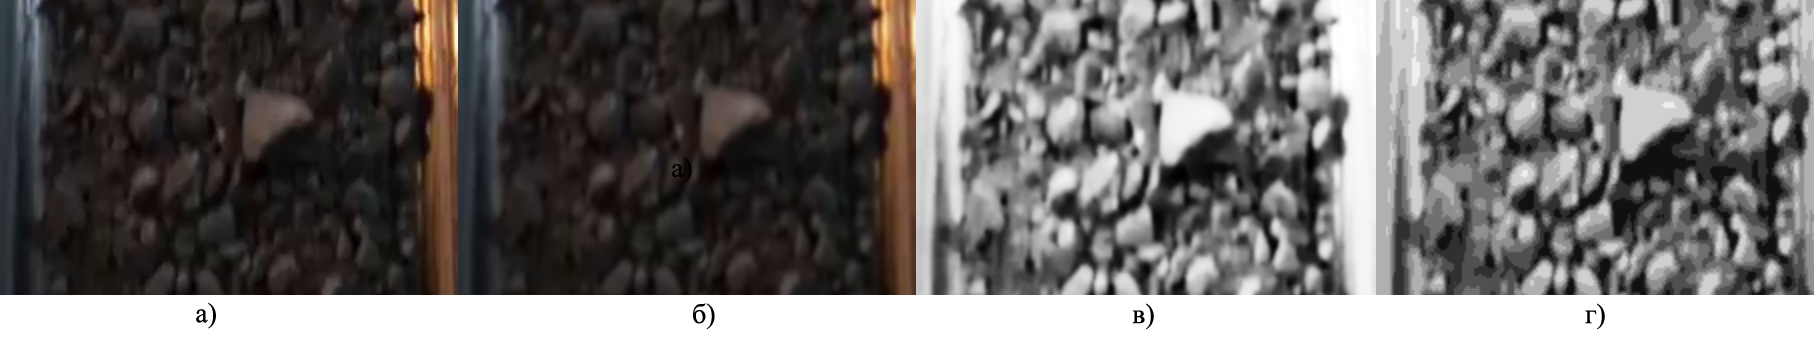
\includegraphics[width=\linewidth]{images/preprocessing}
	\caption{Процесс предобработки изображения: а) исходное изображение, б) изображение после размытие, в) после эквализации гистограммы, г) после уменьшения количества цветов }
	\label{fig:preprocessing}
\end{figure}

\begin{algorithm}[!h]
	\caption{Исходный код функции преобработки:}\label{lst:preprocessing}
	\begin{lstlisting}
	def preprocessing(frame):
	frame = frame[0:700, 130:360]
	cv2_imshow(frame)
	frame = cv2.GaussianBlur(frame,(3,3),0)
	hsv = cv2.cvtColor(frame, cv2.COLOR_BGR2HSV)
	h, s, v = cv2.split(hsv)
	v = cv2.equalizeHist(v)
	hsv = cv2.merge([h, s, v])
	bgr = cv2.cvtColor(hsv, cv2.COLOR_HSV2BGR)
	gray = cv2.cvtColor(bgr, cv2.COLOR_BGR2GRAY)
	div = 32
	gray = gray // div * div + div // 2
	
	return bgr, gray
	\end{lstlisting}
\end{algorithm}

Результатом работы данного этапа является обработанное изображение с повышенной яркостью и уменьшенными шумами. На полученном изображении объекты чётко выделяются на фоне.


\section{Детектирование камней}
Несмотря на то, что технически рассмотренные ниже методы являются методами извлечения признаков и сегментации, но в условиях задачи определения камней уместно называть их методами детектирования камней. Рассмотрим методы сегментации на основе выделения контуров и выращивания регионов. 
\subsection{Алгоритм следования границ}
Стандартным методом определения контуров является метод следования границ (border following). В библиотеке OpenCV именно этот алгоритм реализует функция \texttt{findContour()}. Данный алгоритм чаще всего применяется на бинаризованных изображениях и определяет внешние и внутренние границы контуров объектов путём обхода изображений, находя продолжение контура среди соседей текущего пикселя. Алгоритм позволяет определить иерархию контуров изображения - внешних и внутренних, внутренним контуром считается контур, находящийся внутри другого контура. 

\begin{figure}[h]
	\centering
	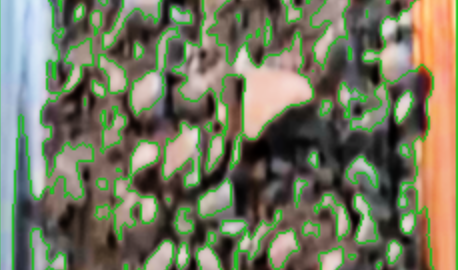
\includegraphics[width=0.6\linewidth]{images/findContour}
	\caption{Результат применения алгоритма следования }
	\label{fig:findcontour}
\end{figure}


В качестве входных данных необходимо использовать 8-битное одноканальное изображение.
Результат применения данного алгоритма к ленте конвейера (рис. \ref{fig:findcontour}) является удовлетворительным, так как алгоритм смог выделить светлые области на изображении, часто совпадающие с камнями, но однако мы можем наблюдать ошибку профиля (рис. \ref{ris:findContours}a) и ошибку разграничения частиц (рис. \ref{ris:findContours}б)

\begin{figure}[h]
	\begin{minipage}[h]{0.49\linewidth}
		\centering
			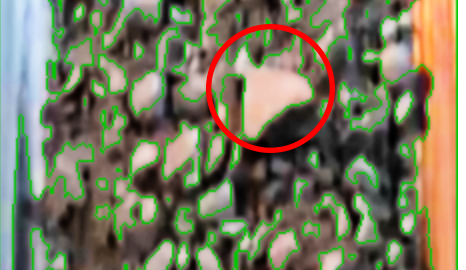
\includegraphics[width=0.9\linewidth]{images/findContour_profile} \\ a)
	\end{minipage}
	\hfill
	\begin{minipage}[h]{0.49\linewidth}
		\centering
		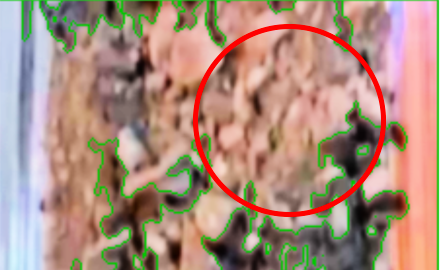
\includegraphics[width=0.9\linewidth]{images/findContours_sep} \\ б)
	\end{minipage}
	\caption{Ошибки, возникшие при применении алгоритма следования границам.}
	\label{ris:findContours}
\end{figure}



\subsection{Алгоритм максимально стабильных экстремальных областей}
Алгоритм максимально стабильных экстремальных областей (MSER) \cite{mser} был реализован для нахождения соответствий между двумя изображения, к одному из которых были применены различных преобразования (например, афинные) на основе того, что экстремальные области у них будут совпадать. Области определяются единственно экстремумом функции интенсивности внутри её и на внешней границ. 

Эту концепцию можно объяснить тем набором возможных пороговых значений бинаризации для уровня серого. При каждом изменении уровня будут формироваться новые регионы, но часть из них останется стабильным на каждом из этих изображений.  Эти регионы и являются максимально стабильными областями. В сочетании с другими методами выделения границ, например, детектором Кенни(пункт \ref{Canny}),можно реализовать достаточно эффективный метод сегментации.

\begin{figure}[h]
	\centering
	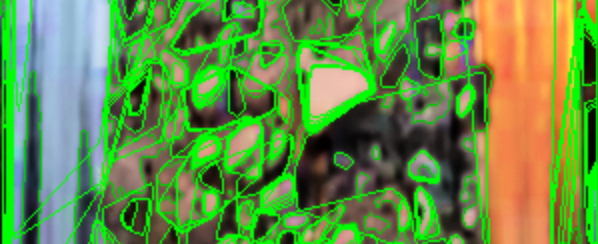
\includegraphics[width=0.6\linewidth]{images/mser1}
	\caption{Результат применения алгоритма MSER}
	\label{fig:mser}
\end{figure}


Рассмотрим применения алгоритма MSER для задачи детектирования камней (рис. \ref{fig:mser}). Результат является неудовлетворительным, так как выделено малое количество камней, а так же наблюдается ошибка профиля (рис. \ref{fig:mser1}a, красный круг), излишняя сегментация (рис. \ref{fig:mser1}a, голубой круг), а так же ошибка разграничения частиц (рис. \ref{fig:mser1}б).

\begin{figure}[h]
	\begin{minipage}[h]{0.49\linewidth}
		\centering
		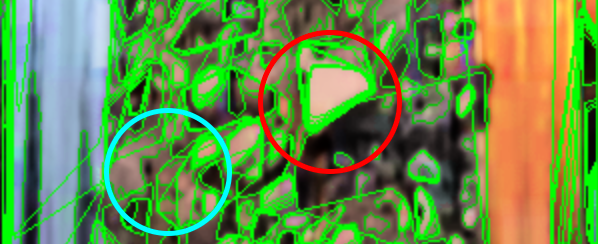
\includegraphics[width=0.9\linewidth]{images/mser2} \\ a)
	\end{minipage}
	\hfill
	\begin{minipage}[h]{0.49\linewidth}
		\centering
		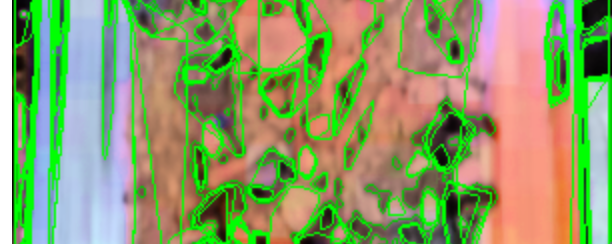
\includegraphics[width=0.9\linewidth]{images/mser3} \\ б)
	\end{minipage}
	\caption{Ошибки, возникшие при применении алгоритма MSER}
	\label{fig:mser1}
\end{figure}

\subsection{Оператор Собеля}\label{Sobel}

Оператор Собеля - дифференциальный оператор, позволяющий вычислить приближённое значение градиента яркости пикселей изображения. Результатом применения оператор Собеля является значение градиента яркости пикселя в каждой точке. Оператор Собеля часто применяется в алгоритмах определения границ. Он основан на свёртке изображения с небольшими ядрами, и хотя градиент вычисляется со значительной погрешностью, но качество аппроксимации является достаточным для решения множества задач. 

В простейшем случае оператор  использует ядра $3x3$ для вычисления свёрток, вычисляя значения первых производных по направлениям. Применение оператора позволяет  определить приближённое значение первой частной производной градиента интенсивности для вертикального и горизонтального направления. На основании этих градиентов возможно вычислить магнитуду градиента для пикселя и направление градиента.  Исходный код вычисления оператора представлен на листинге \ref{lst:sobel}]/

Результатом применение оператора Собеля к изображению (рис. \ref{fig:sobel}) является матрица градиентов, которые примерно показывают расположение камней на конвейере, однако использование для детектирования границ камней только оператора Собеля нецелесообразно. 

\begin{figure}
	\centering
	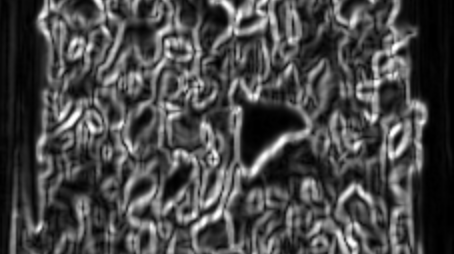
\includegraphics[width=0.7\linewidth]{images/sobel}
	\caption{Результат применения оператора Собеля}
	\label{fig:sobel}
\end{figure}

\begin{algorithm}[h!]
	\caption{Исходный код вычисления оператора Собеля:}\label{lst:sobel}
	\begin{lstlisting}
	scale = 1
	delta = 0
	ddepth = cv2.CV_16S
	grad_x = cv2.Sobel(v, ddepth, 1, 0, ksize=3, scale=scale, delta=delta, borderType=cv2.BORDER_DEFAULT)
	# Gradient-Y
	# grad_y = cv.Scharr(gray,ddepth,0,1)
	grad_y = cv2.Sobel(v, ddepth, 0, 1, ksize=3, scale=scale, delta=delta, borderType=cv2.BORDER_DEFAULT)
	
	abs_grad_x = cv2.convertScaleAbs(grad_x)
	abs_grad_y = cv2.convertScaleAbs(grad_y)
	maskSobel = cv2.addWeighted(abs_grad_x, 0.5, abs_grad_y, 0.5, 0)
	\end{lstlisting}
\end{algorithm}

\subsection{Детектор границ Канни}\label{Canny}
Детектор границ Канни предназначается для поиска границ на изображении. В процессе работы алгоритм Канни самостоятельно удаляет шумы путём применения к изображению фильтрации Гаусса с размером окна 5, и вычисляет первые производные функций интенсивности пикселей посредством оператора Собеля. Полученные градиенты комбинируются к одному из возможных направлений $0, 45, 90$ или $135$ градусов. 

Точки, которые соответствуют локальному максимуму  и соответствующие производным по направлению, становятся кандидатами для группировки в грань контура. Определенные контуры формируются с помощью пороговой функции двойного отсечения (гистерезиса). Если значение градиента в точке выше порога, то эта точка включается в контур, если находится между верхним и нижним порогом, то она принимается как часть грани, только если соединён с точкой, со значением выше порога. Если значение градиента ниже порога, то такая точка отбрасывается. 

\begin{figure}[h!]
	\centering
	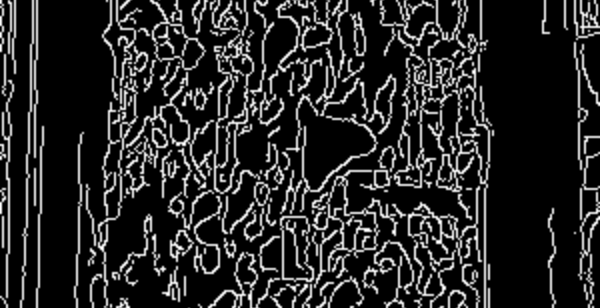
\includegraphics[width=0.7\linewidth]{images/canny}
	\caption{Результат применения детектора границ Канни}
	\label{fig:canny}
\end{figure}

Результат применения детектора границ Канни к изображению (рис. \ref{fig:canny}) ленты конвейера не позволяет чётко выделить камни, однако, может быть полезен в качестве дополнительных исходных данных для других методов. 

\subsection{Метод водораздела}
 Существуют два ключевых подхода к сегменментации: на основе выделения границ и на основе метода выращивания регионов, а так же смешанный подход.
Простые методы не могут эффективно решить задачу детектирования камней на плоскости, однако, их использование эффективно в качестве этапов сегментанции. Метод водораздела относится к методам выращивания регионов и является одним из самых популярных и эффективных методов сегментации\cite{watershed}.

Суть метода водораздела заключается в обнаружении маркеров \cite{watershedmarker}, которые будут являться точками локального минимума, точек, находящихся на возвышенности и точек, находящихся на склоне, с которых вода разных цветов будет сливаться к центру водоёма. 

Алгоритм работы метода водораздела следующие:
\begin{enumerate}
	\item  В местах локального минимума образуются отверстия, через которые вода начинает заполнять поверхность.
	\item Eсли вода с двух сторон возвышенности готова слиться в один бассейн, то необходимо установит перегородку между бассейнами.
	\item Когда вода заполнит всё изображение, то алгоритм можно остановить.
\end{enumerate}


Использование водораздела часто приводит к сильной сегментации, поэтому чаще всего используется водораздел на основе маркеров.  Маркер являет собой точку локального минимума, на основе которого будет выбран бассейн. Маркеры возможно расставлять как вручную, так и автоматически.

Процедура выбора маркеров построена следующим образом:
\begin{enumerate}
	\item предобработка;
	\item выбор критерия, по которому определяется маркер;
	\item выявление маркеров.
\end{enumerate}

Способ ручной установки маркеров не подходит для данной задачи гранулометрии, так как число камней на одном изображении - больше ста, а алгоритм должен работать в режиме реального времени. Поэтому рассмотрим способ автоматической расстановки маркеров на изображении конвейера. 

Первым этапом для вычисления маркеров является использование морфологической операции "размыкание"\cite{opening}, позволяющее выявить объекты переднего плана, так как оно сглаживает границы объектов, приводя их к размеру окна. В случае данной задачи оптимальным было признано использование размера окна $(5x5)$. Результат применение операции приведён на рис. \ref{fig:opening}.

\begin{figure}[h!]
	\centering
	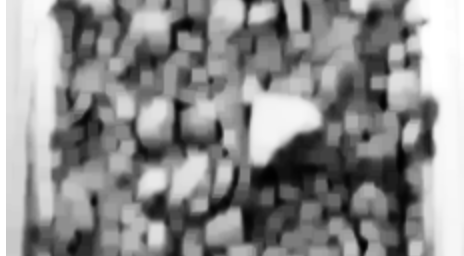
\includegraphics[width=0.5\linewidth]{images/opening}
	\caption{Результат применения операции размыкание}
	\label{fig:opening}
\end{figure}

Следующим шагом является применение адаптивной бинаризации. Часто используют пороговую бинаризацию, считающую все пиксели, значения которых выше порога - белыми, а которых ниже - чёрными, но этот метод не всегда эффективен, если яркость изображения неоднородна.

\begin{figure}[h!]
	\centering
	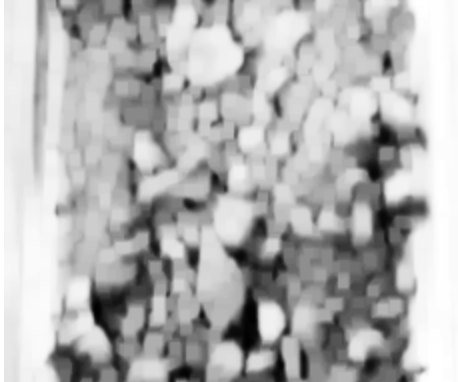
\includegraphics[width=0.5\linewidth]{images/overlightning}
	\caption{Засвет в верхней части}
	\label{fig:overlightning}
\end{figure}


 В случае фотографии конвейера выравнение гистограммы в верхней части образовывался засвет, из-за которого не удавалось чётко сегментировать объекты в верхней части - после бинаризации невозможно было выделить маркеры. Адаптивная бинаризация определяет порог на окружающих пикселей. Размер окна задаётся параметрами бинаризации. Результат бинаризации представлен на рис. \ref{fig:binary}. 


\begin{figure}[h!]
	\centering
	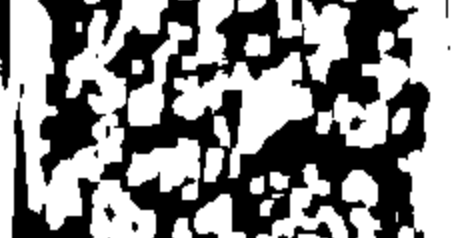
\includegraphics[width=0.6\linewidth]{images/binary}
	\caption{Результат бинаризации}
	\label{fig:binary}
\end{figure}


Последним этапом вычисления маркеров является дистанционная трансформация, принимающая в качестве входных значений бинаризованное изображение, и вычисляющая новые значения интенсивностей пикселя на основе удаления от ближайшей границы. Точка с максимальной интенсивностью является локальным минимумом области, и является маркером (рис. \ref{fig:markers}).  

\begin{figure}[h!]
	\centering
	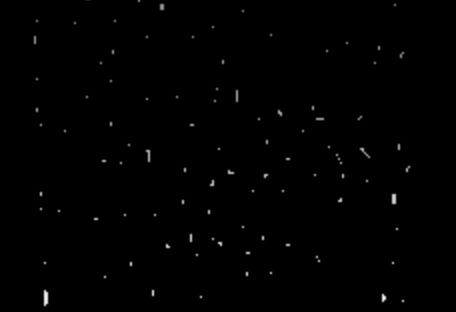
\includegraphics[width=0.6\linewidth]{images/markers}
	\caption{Полученные маркеры}
	\label{fig:markers}
\end{figure}

Для повышения точность водораздела его комбинируют c одним из методов выявления границ. Лучший результат показало использование в качестве маски изображение, обработанного оператором Собеля.После вычисления бассейнов границы определяются с помощью алгоритма следования границам.  Результат маркерного водораздела (рис. \ref{fig:final}). Несмотря на наблюдаемые ошибки разграничения частиц, маркерный водораздел показывает лучшие результаты, чем определения границ.

\begin{figure}[h!]
	\centering
	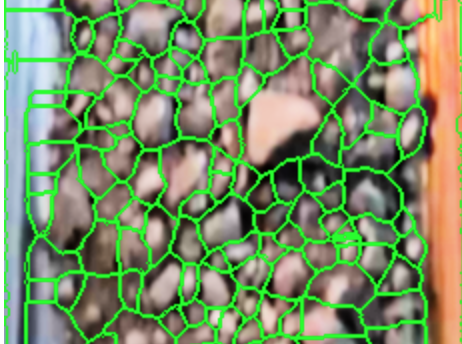
\includegraphics[width=0.6\linewidth]{images/final}
	\caption{Результат использования маркерного водораздела и оператора Собеля.}
	\label{fig:final}
\end{figure}

\section{Детектирование с помощью нейронной сети U-net}
Рассмотренные выше алгоритмы детектирования с использованием классических методов компьютерного зрения показывают хороший результат, однако с помощью классических преобразований возникают ошибки детектирования в сложных местах. Поэтому исследуем применимость нейронных сетей для детектирования камней. 
\subsection{Нейросеть U-net}
U-Net считается одной из стандартных архитектур свёрточных нейронных сетей, используемых для задач сегментации изображений \cite{unet}. Особенность данной нейронной сети в том, что она позволяет сегментировать область по классу, т.е., создать маску, позволяющую разделить изображение на несколько классов. U-Net  была разработана в 2015 году для сегментации биомедицинских изображений в Фрайбургском университете. Так же был найден результат использования данной нейросети для задачи определения камней \cite{unerrock}

Архитектура сети (рис. \ref{fig:unet}) представляет собой полносвязную свёрточную сеть, модифицированную так, чтобы она могла работать с меньшим количеством примеров (обучающих образов) и позволяла осуществлять более точную сегментацию по классам. 

Основная идея состоит в том, чтобы дополнить обычную сеть последовательными уровнями, где операции объединения заменяются операторами с повышением частоты. Следовательно, эти слои увеличивают разрешение на выходе. Более того, следующий сверточный слой может затем научиться собирать точные выходные данные на основе этой информации.


\begin{figure}
	\centering
	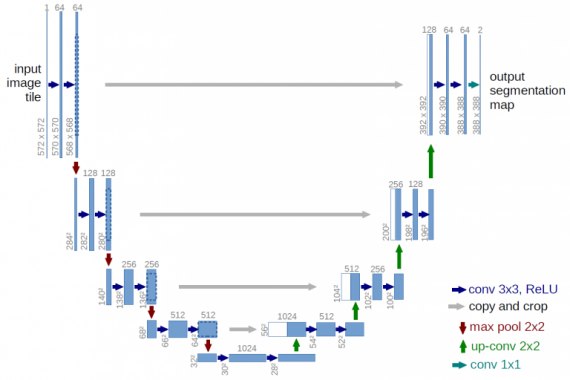
\includegraphics[width=\linewidth]{images/unet}
	\caption{Архитектура нейронной сети Unet}
	\label{fig:unet}
\end{figure}


Обучение в нейронных сетях достигается за счёт минимизации функции потерь. В данном случае unet в качестве функции потерь часто используется бинарная кроссэнтропия. Бинарная кроссцентропия измеряет, насколько далеко от истинного значения (равного 0 или 1) предсказание для каждого из классов, а затем усредняет эти классовые ошибки, чтобы получить окончательную потерю.

\subsection{Обучение сети}
Для оценивания, подходит ли нейронная сеть U-net для данной задачи было произведено обучение на обучающей выборке,  собранной с помощью метода водораздела. Полученные регионы для данной задачи целесообразно наложить на маску, полученную с помощью адаптивной бинаризацией, так как таким образом мы получим не разбиение на регионы, а выделение конкретных камней, что позволит создать маску (рис. \ref{fig:dataset}) Однако данная выборка имеет области, где несколько камней сливаются в один, а так же области ограждения конвейера, тоже попавшие в маску.

Для обучения использовалось 50 изображений. Исходная выборка была увеличена путём аугментации\cite{dataaug}. Аугментация - модификация исходных данных путём примения к ним аффинных преобразований и работы с цветом. Аугментация позволяет повысить качество обучение модели. 


\begin{figure}[h!]
	\begin{minipage}[h]{0.49\linewidth}
		\centering
		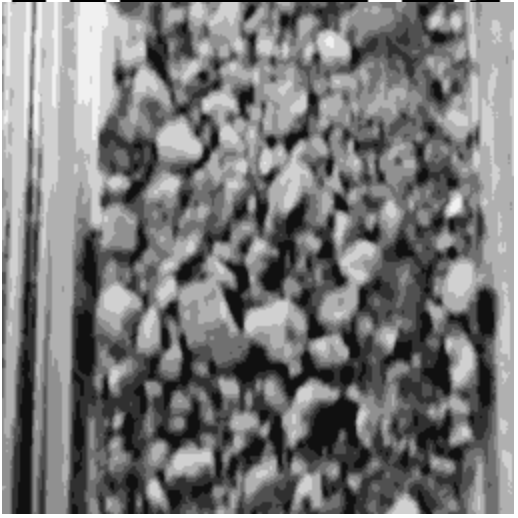
\includegraphics[width=0.9\linewidth]{images/train1} \\ a)
	\end{minipage}
	\hfill
	\begin{minipage}[h]{0.49\linewidth}
		\centering
		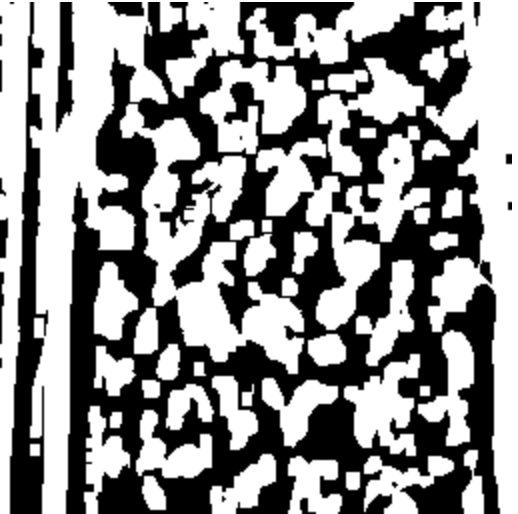
\includegraphics[width=0.9\linewidth]{images/train2} \\ б)
	\end{minipage}
	\caption{Данные датасета для обучения}
	\label{fig:dataset}
\end{figure}

Нейронная сеть была обучена в течение 5 эпох по 1000 шагов в каждой. Полученное значение функции потерь  - 0.15, полученная точность - 0.91. Результат работы нейронной сети сравним с результатом работы классических методов (рис. \ref{fig:result}). Результат обработанных изображений сравним с классическими методами обработки, поэтому целесообразно модифицировать обучающую выборку и продолжить исследование.

\begin{figure}[h!]
	\begin{minipage}[h]{0.49\linewidth}
		\centering
		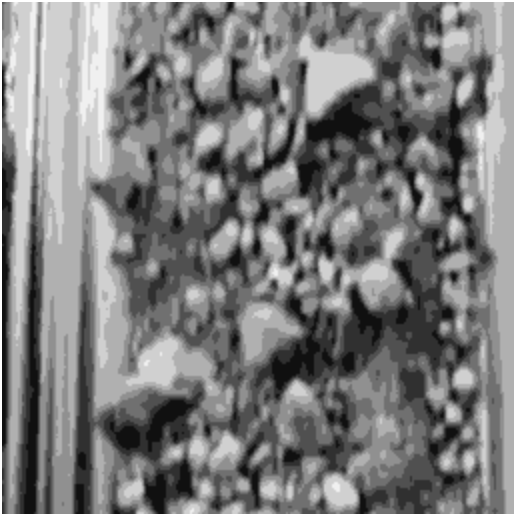
\includegraphics[width=\linewidth]{images/test1} \\ a)
	\end{minipage}
	\hfill
	\begin{minipage}[h]{0.49\linewidth}
		\centering
		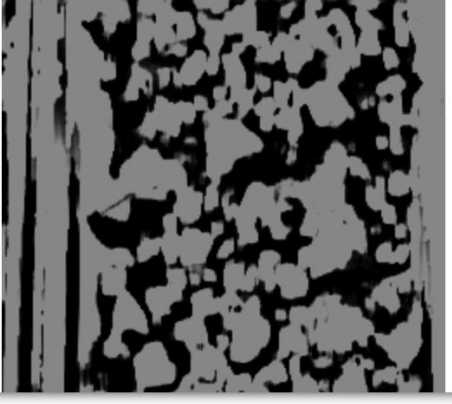
\includegraphics[width=\linewidth]{images/test2} \\ б)
	\end{minipage}
	\caption{Результат работы нейронной сети, обученной на автоматически собранном датасете.}
	\label{fig:result}
\end{figure}

Изображения обучающей выборки были модифицированы с использованием графического редактора (рис. \ref{fig:newdataset}). Убраны ошибочно выделенные объекты, такие как детали конвейера, убраны распознанные как крупные камни области песка (ошибка разделения мелких частиц), выделены границы для нескольких камней, распознанных как один, или убраны для камней, распознанных как несколько.

 \begin{figure}[h!]
 	\begin{minipage}[h]{0.49\linewidth}
 		\centering
 		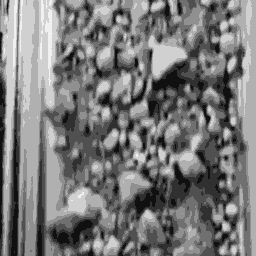
\includegraphics[width=\linewidth]{images/train3} \\ a)
 	\end{minipage}
 	\hfill
 	\begin{minipage}[h]{0.49\linewidth}
 		\centering
 		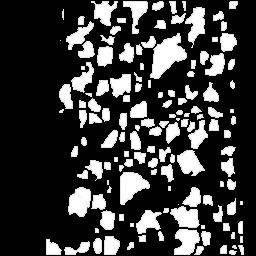
\includegraphics[width=\linewidth]{images/train4} \\ б)
 	\end{minipage}
 	\caption{Исправленный датасет для обучения.}
 	\label{fig:newdataset}
 \end{figure}
 
 Экспериментальным образом было подобрано время обучение в течение 5 эпох и 2000 шагов в каждой эпохе. Полученное значение функции потерь 0.15, полученная точность - 98.5\%. Проверим результат работы алгоритма на тестовой выборке, не пересекающейся с обучающей (рис. \ref{fig:unetresult}). В результате обучения нейронная сеть достаточно точно детектирует камни, распознавая около 90\% камней, так же игнорируя ленты конвейера. Относительно классических методов компьютерного зрения, нейронная сеть обучена таким образом, что не выделяет области мелких камней как один большой камень (ошибка разграничения частиц), что является плюсом. Однако,при использовании этого метода,  как и все методов, использующие двумерные изображения, сложно избежать ошибку профиля.  
 
  \begin{figure}[h!]
 	\begin{minipage}[h]{0.3\linewidth}
 		\centering
 		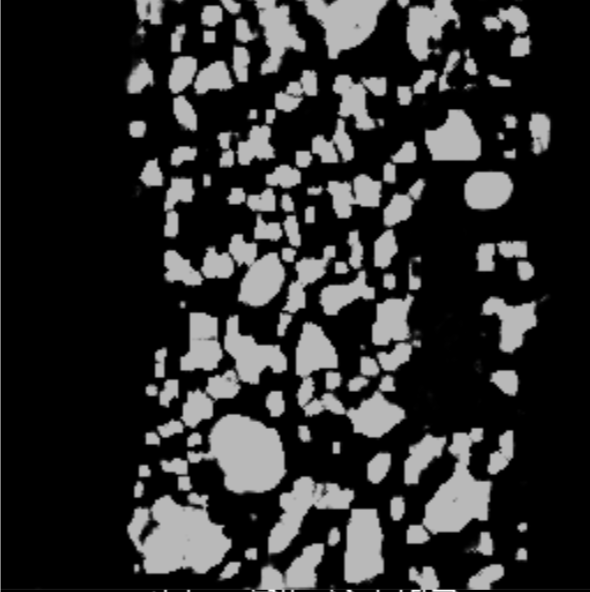
\includegraphics[width=\linewidth]{images/unetmask} \\ a)
 	\end{minipage}
 	\hfill
 	\begin{minipage}[h]{0.3\linewidth}
 		\centering
 		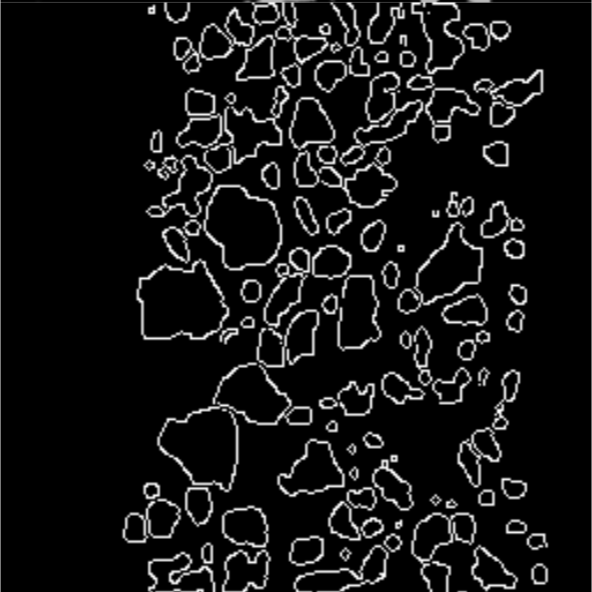
\includegraphics[width=\linewidth]{images/unetcanny} \\ б)
 	\end{minipage}
  	\hfill
 	\begin{minipage}[h]{0.3\linewidth}
 	\centering
 	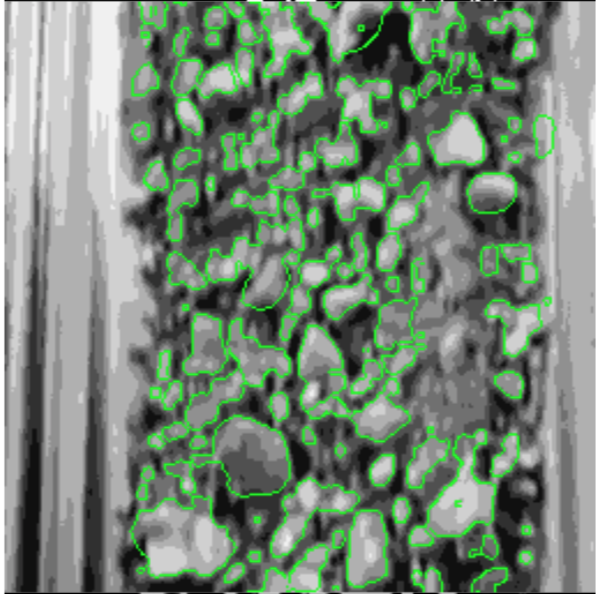
\includegraphics[width=\linewidth]{images/unetresult} \\в)
 \end{minipage}
 	\caption{Полученные результаты. а) полученная маска б) выделение границ полученной маски в) совмещение маски и исходного изображения}
 	\label{fig:unetresult}
 \end{figure}

\chapterconclusion
В данной главе производилось исследование различных методов сегментации на основе классичесских методов компьютерного зрения с использованием детектирования границ (Алгоритм следования за границами, детектор Канни, оператор Собеля, метод максимальных стабильных экстермальных областей) и метода выращивания регионов (метод водозраздела). Лучший результат из классических методов показывает метод маркерного водораздела с маской, построенной с использованием оператора Собеля. При использовании методов классического компьютерного зрения сложно избежать ошибку разграничения частиц. 
На основе данных, собранных путём метода водораздела, возможно собрать обучающую выборку, вручную отредактиров фотографии, и обучив с использованием нейронной сети для сегментации Unet. При сегментации с использованием нейронной сети повышается точность детектирования и исчезает проблема разделения частиц .


\chapter{Алгоритмы оптического потока}
В данной главе исследуется применение различных методов оптического потока для построения распределения камней по конвейеру. Оптический поток часто используется для отслеживания движения, и реже - но тоже используется, для сегментации изображения. 
\section{Понятие оптического потока}
Оптический поток  - модель видимого движения объектов, поверхностей и краев в окружении,  созданная на основе относительного движения между наблюдателем и сценой. 
Оптический поток определяют как видимое смещение отдельных пикселей на плоскости изображения. Иными словами, оптический поток показывает движение набора пикселей, обычно являющихся одним объектом, на фоне. 

Концепция оптического потока представляет собой матрицу скоростей (т. к. сдвиг  эквивалентен мгновенной скорости). Для каждой точки изображения $I_{1}(x,y)$ можно найти такой сдвиг $(dx, dy)$, чтобы исходной точке соответствовала какая-либо точка второго изображения $I_{2}(x+dx,y+dy)$.
Соответствие точек возможно определить благодаря тому, что вместо цвета пикселя используется какая-либо функция этого пикселя, которая не будет изменяться в течение времени, например, интенсивность. Однако, значение интенсивности может резко изменяться при резкой смене освещение, но считается, что в видеоряде между двумя кадрами значение освещённости пикселя не будет резко изменяться.

Часто результат вычисления оптического потока служит хорошим приближением к истинному физическому движению, спроецированному на плоскость изображения. Большинство методов, которые вычисляют оптический поток, предполагают, что цвет или интенсивность пикселя инвариантны при смещении от одного видеокадра к следующему. 

Существуют два варианта вычисления оптического потока:
\begin{enumerate}
	\item Плотный (dense), оптический поток рассчитывает смещение всех пикселей изображения.
	\item Разреженный (sparce), оптический поток рассчитывает смещение только некоторых заданных точек, например, выделенных краёв или маркеров.
\end{enumerate}

Существуют несколько подхода к визуализации оптического потока:
Для визуалиции разреженного оптического потока чаще всего производится построение траектории движения объекта на основе перемещения ключевых точек. Для плотного потока возможна визуализация цветом (рис. \ref{fig:flow}a) на основе вычисленных значений векторов или построение векторов с заданным шагом  (рис. \ref{fig:flow}б). 

Математически в общем случае оптический поток описывается следующим образом:
Пусть  $I_1 = I(x, y, t)$ – интенсивность пикселя некоторого пикселя $(x, y)$ на первом изображении (т. е. в момент времени t). На втором изображении эта точка сдвинулась на $(dx, dy)$, при этом прошло время $dt$, тогда $I_2 = (x+dx, y+dy, t_1+dt) ~ I_1 + I_xdx +I_ydy+I_tdt$, $I_{x},I_{y},I_{t} $– частные производные по координатам и времени, и $I_{t}dt$ – является изменение яркости в точке $(x, y)$  между двумя кадрами.

Так как мы предполагаем, что интенсивность имеет постоянное значение, то $I_{1}=I_{2}\Rightarrow  I_xdx +I_ydy+I_tdt = 0$. В таком случае мы получаем уравнение с двумя неизвестными $(dx и dy)$, которого недостаточно для решения, однако различные методы предлагают подходы к решению.

\begin{figure}[h]
	\begin{minipage}[h]{0.49\linewidth}
		\centering
		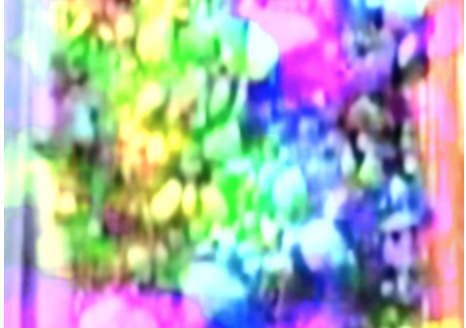
\includegraphics[width=0.9\linewidth]{images/color} \\ a)
	\end{minipage}
	\hfill
	\begin{minipage}[h]{0.49\linewidth}
		\centering
		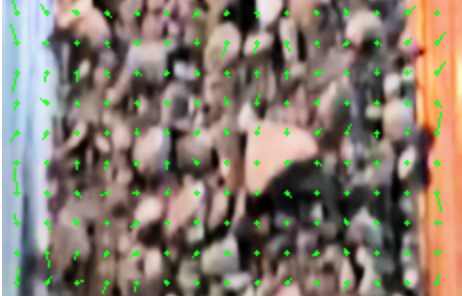
\includegraphics[width=0.9\linewidth]{images/vector} \\ б)
	\end{minipage}
	\caption{Отображение оптического потока}
	\label{fig:flow}
\end{figure}


\section{Алгоритм Лукаса-Канаде}

Оптический поток по методу Лукаса-Канаде является стандартным и самым простым методом вычисления оптического потока.

Объекты на изображении точноимеют размеры больше, чем 1 пиксель, в таком случае, вероятно, что в окрестности конкретного пикселя другие точки будут иметь схожие сдвиги. В таком случае, если взять окно вокруг этого пикселя и минимизировать по методу наименьших квадратов суммарную погрешность с весовыми коэффициентами, имеющими распределение по Гауссу, то есть, чтобы ближайшие пиксели к исследуемому имели наибольший вес. После преобразований получаем систему из двух уравнений с двумя неизвестными.
\begin{eqnarray}
\sum_{i, j} g(x, y) I_x(x_i, y_j )^2 dx + \sum_{i, j} g(x, y) I_x(x_i, y_j ) I_y(x_i, y_j ) dy 
\nonumber \\  = - \sum_{i, j} g(x, y) I_x(x_i, y_j ) I_t(x_i, y_j )^2 dt;  \\
\sum_{i, j} g(x, y) I_x(x_i, y_j ) I_y(x_i, y_j ) dx + \sum_{i, j} g(x, y) I_x(x_i, y_j )^2 dy \nonumber
\\ = - \sum_{i, j} g(x, y) I_x(x_i, y_j ) I_t(x_i, y_j )^2 dt.
\end{eqnarray}

Cистема чаще всего имеет единственное решение, однако, если детерминант системы равен нулю, то решений либо не существует, либо имеется бесконечное количество. Эта проблема известна как Aperture problem – неоднозначность сдвига при ограниченном окне для периодических изображений. В таком виде алгоритм Лукаса-Канаде хорошо определяет маленькие сдвиги, такие, в рамках которых изображение похожа на свое линейное приближение. 

Чтобы сделать алгоритм более универсальным, используется multi-scaling: строится «пирамида» изображений разного масштаба (в основном производится масштабирование в 2 раза по каждой оси). Оптический поток вычисляется на всех изображениях от меньшего к большему, и  детектированный маленький сдвиг на маленьком изображении будет соответствовать большому сдвигу на большом изображении. На изображении самого меньшего масштаба обнаруживается сдвиг не более 1-2 пикселей, а при переходе от меньшего масштаба к большем  используется результат предыдущего шага и проиходит уточнение значения сдвига. 

Использование этого пирамидального алгоритма позволяет не вычислять линейную аппроксимацю по большому количеству точек: берётся множество уровней пирамиды, и на каждом уровне берётся грубое приближение этой функции. В OpenCV  идет расчет всего по двум соседним точкам. 

Применим  алгоритм Лукаса-Канаде к видео с конвейера. Алгоритм Лукаса-Канаде вычисляет разреженный оптический поток, то есть для заданного набора точек на первом изображении оценивает их положение на втором., поэтому изначально выделяют точки для отслеживания. В нашем случае выделим их с помощью функции \texttt{cv2.goodFeaturesToTrack}. В качестве входных данных для алгоритма используются: 2 изображения - предыдущий кадр и текущий, размер окна для усреднения по Гауссу, количество слоев в пирамиде. Оставим размер окна и количество слоёв по умолчанию. Получаенный результат (рис. \ref{fig:lk}) является неудовлетворительным, так как отслеживаются не все камни, и сложно на основе значений выделить изображения камней. Сделаем вывод, что разреженный поток не подходит для нашей задачи.

\begin{figure}[h!]
	\centering
	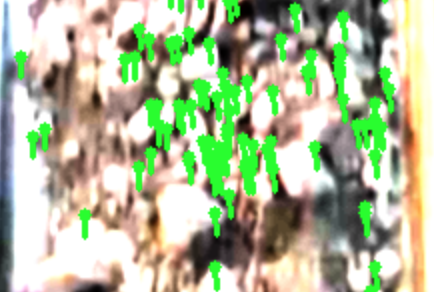
\includegraphics[width=0.7\linewidth]{images/lk}
	\caption{Результат применения алгоритма Лукаса-Канаде.}
	\label{fig:lk}
\end{figure}


\section{Алгоритм Фарнебэка}

Метод, представленный Гуннаром Фарнэбэком аппроксимирует окна кадров изображения квадратичными полиномами с помощью преобразования полиномиального расширения. При наблюдении полиномиального преобразования при перемещении  оцениваются вектора смещения на основе коэффициентов полиномиального расширения. После ряда уточнений вычисляется плотный оптический поток.

У этого алгоритма есть модификации и усовершенствования, в первую очередь позволяющие использовать известную априорную информацию – заданную начальную аппроксимацию потока и multi-scaling.

Для реализации в библиотеке OpenCV он вычисляет величину и направление оптического потока на основе двухканального массива векторов потока $(dx/dt, dy/dt)$. Затем он визуализирует направление потока по оттенку и величину потока по значению цветового представления HSV. Размерность HSV всегда установлена на максимум 255 для оптимальной видимости.

Алгоритм Farneback реализуется функцией calcOpticalFlowFarneback. Алгоритм рассчитывает сплошной поток, то есть сдвиг каждой точки. В качестве параметров используется: входные изображения (предыдущее и текущее), отношение масштабов между слоями пирамиды (стандартное значение 0.5), количество уровней в пирамиде,  размер окна, по которому производится усреднение,  количество итераций на каждом уровне пирамиды, размер полинома, по которому оцениваются значения матрицы, сигма гауссовского размытия при сглаживании производных, рекомендованные значения параметров указаны в мануале. 

Применим алгоритм Фарнэбэка к видео с конвейера. Используем значения, рекомендованные в мануале. В первую очередь попробуем определить, будет ли наблюдаться различное смещение относительно предыдущего кадра (рис.\ref{fig:farn}a), и видим, что алгоритм распознается смещение множества камней как смещение с одинаковой интенсивностью, то есть выделить отдельные камни невозможно. В таком случае попробуем рассчитать смещение относительно фонового кадра (рис.\ref{fig:farn}б), и видим, что можно выделить отдельные области, однако, они совпадает с несколькими кучами камней. Сегментация камней на основе этих данных невозможна.

\begin{figure}[h]
	\begin{minipage}[h]{0.49\linewidth}
		\centering
		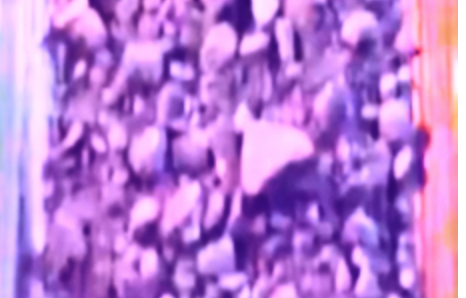
\includegraphics[width=0.9\linewidth]{images/pink} \\ a)
	\end{minipage}
	\hfill
	\begin{minipage}[h]{0.49\linewidth}
		\centering
		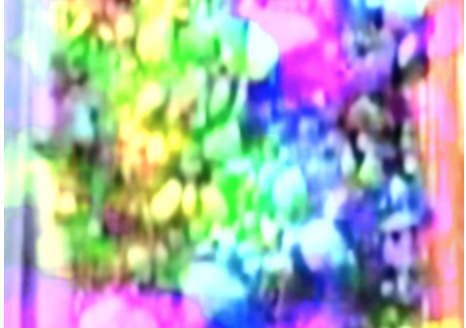
\includegraphics[width=0.9\linewidth]{images/color} \\ б)
	\end{minipage}
	\caption{Результат работы алгоритма Farneback. }
	\label{fig:farn}
\end{figure}


\section{Алгоритм Simple flow}
В основе метода SimpleFlow\cite{sf} лежит концепция поиска максимально похожей точки на следующем кадре, так как в условиях того, что мы не сможем определить сдвиг  пикселя больше размера окна, по которому ищут производные. Для разрешения неоднозначностей и уменьшения шумом будет считать, что поток непрерывность, и в окрестности определённого нам пикселя все пиксели имеют схожий сдвиг. Так же ограничение размера окна компенсируется, используя приём multi-scaling.

Применением алгоритм к задаче сегментации камней. Алгоритм SimpleFlow реализует функция calcOpticalFlowSF. Алгоритм так же реализует dense поток.  В качестве параметров алгоритм принимает входные изображения, количество слоёв в пирамиде, размер окна, максимальный возможный сдвиг пикселя. Данный алгоритм достаточно долго обрабатывает один кадр - около 2 секунд. При использовании двух соседних кадров мы так же не наблюдаем различного смещения (рис. \ref{fig:sf}), но при использовании в качестве базового кадра-маски мы можем видеть, что алгоритм выделяет различные области на основе оцениваемого смещения. Однако, при наложении алгоритма детектирования мы можем видеть, что точная оценка работы алгоритма не имеет смысла, так как согласно визуальной алгоритм не выделяет конкретные области.

\begin{figure}[h]
	\begin{minipage}[h]{0.49\linewidth}
		\centering
		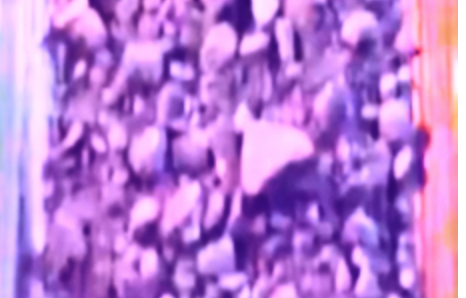
\includegraphics[width=0.9\linewidth]{images/pink} \\ a)
	\end{minipage}
	\hfill
	\begin{minipage}[h]{0.49\linewidth}
		\centering
		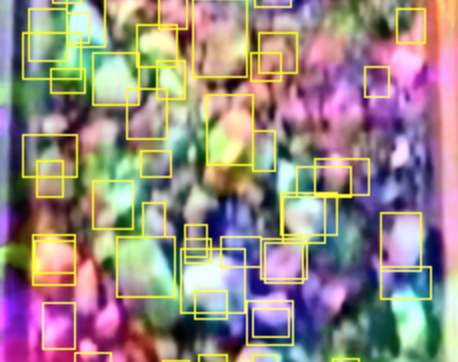
\includegraphics[width=0.9\linewidth]{images/sf} \\ б)
	\end{minipage}
	\caption{Результат работы алгоритма Simple flow. }
	\label{fig:sf}
\end{figure}


 \chapterconclusion
Оптический поток является перспективным методом для сегментации объектов на видео. В данной главе были исследованы алгоритмы Лукаса-Канаде, Фернэбэка и SimpleFlow, однако не один из этих методов не смог достичь точности методов детектирования, описанных в главе \ref{detecting}. Можно сделать вывод, что применение оптического потока нецелесообразно для решения задачи гранулометрии.


\chapter{Алгоритмы отслеживания объектов}

Отслеживание объектов - область исследований компьютерного зрения, занимающаяся определением местоположения движущегося объекта при изменении во времени. Алгоритмы анализируют кадры видео и обновляет высчитанные координаты выделенного объекта. В условиях задачи гранулометрии отслеживание камней может быть полезно для определения необходимой частоты детектирования.  Отслеживание является более быстрой задачей чем детектирование, так как при выполнении операции отслеживания у нас есть информация об объекте с предыдущего кадра, и хороший алгоритм будет использовать всю информацию с предыдущих кадров. Поэтому при разработке эффективной системы операция детектирования выполняется раз в $N$, в то время как операция отслеживания в кадрах между ними. 

В качестве алгоритмов отслеживания для исследования были выбраны:
\begin{itemize}
	\item алгоритм  Multiple Instance Learning (MIL);
	\item алгоритм корреляционного трекера;
	\item центроидный трекер.
\end{itemize}

\section{Отслеживание с использованием обучения  с использованием  нескольких экземпляров}
Обучение  с использованием  нескольких экземпляров (MIL) - это структура, в которой обучающие примеры предоставляются в виде маркированных пакетов, а не маркированных экземпляров. 
MIL - это форма обучения со слабым контролем.  Вместо того чтобы получать набор экземпляров с индивидуальной метками, учащийся получает набор помеченных пакетов, каждый из которых содержит множество объектов. В простом случае двоичной классификации нескольких экземпляров набор может быть помечен как негативный, если все экземпляры в нем негативные. С другой стороны, набор помечается как положительная, если в ней есть хотя бы один положительный экземпляр. Из коллекции маркированных пакетов учащийся пытается либо создать модель, которая будет правильно помечать отдельные экземпляры, либо  научиться размечать наборы без использования модели.  

Алгоритм MIL обучает классификатор в режиме онлайн, чтобы отделить объект от фона. MIL позволяет избежать проблемы смещения для надежного отслеживания.

\begin{figure}
	\centering
	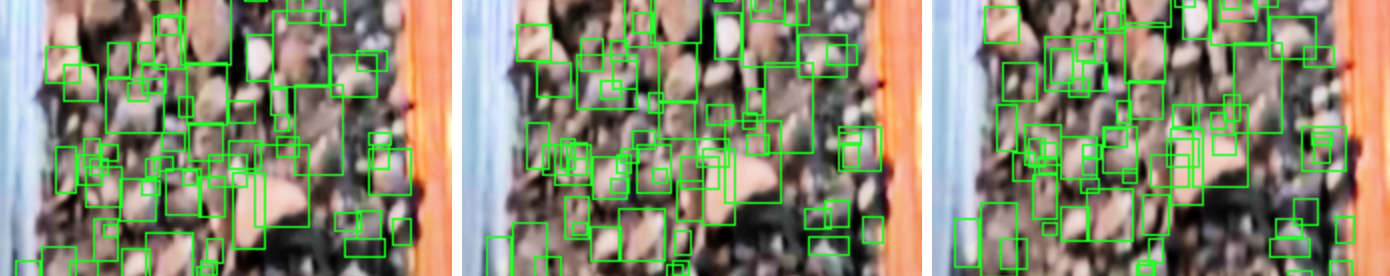
\includegraphics[width=\linewidth]{images/corr}
	\caption{Результат работы MIL-трекера.}
	\label{fig:corr}
\end{figure}

В качестве входных данных для алгоритма подается массив наборов кооррдинат рамок, окружающих объекты. Для каждого кадра вычисляется новое положение объекта. Алгоритм MIL справляется с отслеживанием камней на конвейере (рис. \ref{fig:corr}) и имеет высокую точность (не отслеживаются только ~5\% самых мелких камней), однако мы можем наблюдать ошибку накопления трекеров (рис. \ref{fig:corrsumm}), из-за которой необходимо обновлять трекеры раз в некоторое количество кадров.  


\begin{figure}[h!]
	\centering
	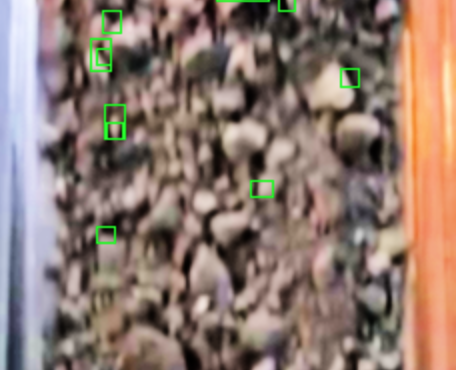
\includegraphics[width=0.5\linewidth]{images/mil_donttrack}
	\caption{Неотслеженные объекты алгоритма MIL.}
	\label{fig:mildonttrack}
\end{figure}


Так же алгоритм MIL обрабатывает один кадр с более десяти секунд, что не позволяет использовать его для обработки кадров в реальном времени, время обработки значительно превышает время детектирования.  Такое время обработки возникает из-за большого количества (более 200) объектов в кадре. 
Из 245 объектов в кадре тестового участка видео неотслеженными оказались 7 (рис. \ref{fig:mildonttrack}), что подтверждает высокую точность алгоритма. 


\begin{figure}[h!]
	\centering
	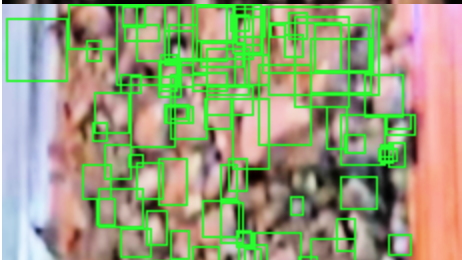
\includegraphics[width=0.5\linewidth]{images/mil_summ}
	\caption{Ошибка накопления трекеров MIL-трекера.}
	\label{fig:corrsumm}
\end{figure}

Были выявлены следующие положительные стороны:
\begin{itemize}
	\item высокая точность отслеживания;
\end{itemize}
Были выявлены следующие проблемы:
\begin{itemize}
	\item снижение скорости из-за накопления трекеров;
\item  	необходимость запускать детектирование новых объектов;
\item 	сброс существующих трекеров при детектировании новых.
\item 	отсутствие автоматическое очищение треков при пропадании из кадра.
\end{itemize}



\section{Корреляционное отслеживание }
 Реализация алгоритма корелляционного трекера \cite{corrtrack} базируется на алгоритме MOSSE (Minimum Output Sum of Squared Error Filter), а именно на дискриминативных корпеляционных фильтров, предлагает использовать масштабную пирамиду, чтобы точно оценить масштаб объекта после того, как было найдено оптимальное отражение.  
 
 Корреляция между изображения описывается достаточно простой концепцией. При ипользования изображение, описываемого функцией $f(x, y)$, задача определения корреляции заключается в нахождении областей изображения, лучше всего соответствующих маске. Маской или эталону соответствуется заданное подизображение $w(x,y)$.
 
 В общем случае корреляционные трекеры определяют изменение положения объекта, используя фильтры, обученные на тренировочных изображениях. На этапе инициализации выбирается цель на основе небольшого окна слежения, расположенного по центру объекта в первом кадре. 
 
 После этапа инициализации обучение и обновление трекера работают одновременно. Цель сопровождается на основании корреляции. Максимальное значение корреляции  при минимальной сумме квадратичной ошибки определяет новые координаты объекта. 
 
 В качестве входных данных для алгоритма подается массив наборов кооррдинат рамок (прямоугольников), окружающих объекты. Для каждого кадра вычисляется новое положение объекта. 
Скорость обработки у алгоритма корреляционного отслеживания гораздо выше, чем у алгоритма обучения с использованием нескольких экземпляров,  однако точность значительно ниже (рис. \ref{fig:correrr}, представлены неотслеживаемые объекты). На обработку одного кадра уходит около 2 секунд. 

\begin{figure}
	\centering
	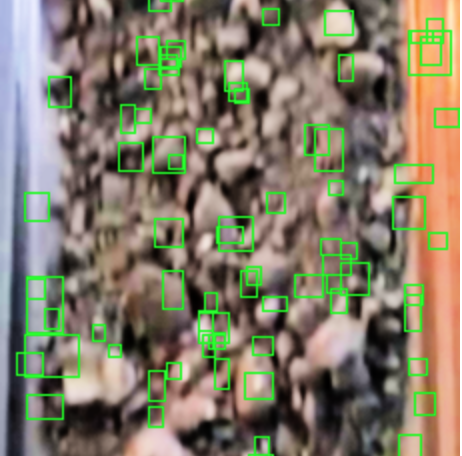
\includegraphics[width=0.5\linewidth]{images/corr_err}
	\caption{Ошибка отслеживания корреляционного трекера}
	\label{fig:correrr}
\end{figure}


Были выявлены следующие положительные стороны:
\begin{itemize}
	\item достаточно высокая скорость обработки кадра.
\end{itemize}
Были выявлены следующие проблемы:
\begin{itemize}
\item снижение скорости из-за накопления трекеров;
\item низкая точность;
\item необходимость запускать детектирование новых объектов;
\item накопление треков исчезнувших объектов в кадре до очищения;
\item  сброс существующих трекеров при детектировании новых.
\end{itemize}

\section{Отслеживание с использование центроидного трекера}
Центроидный трекер  используется в дополнение к любому методу отслеживания объектов как дополнительный. Использование центроидного трекера позволяет решить проблему накопления треков исчезнувших объектов в кадре.
 Он принимает начальные координаты прямоугольника, описывающего объекты и формирует объект центроида. Каждому центроиду присваивается новый идентификатор. После обновления кадра вычисляется евклидово расстояние между новыми ограничительными рамками и существующими объектами, и на основе минимального расстояния объектам присваиваются старые или новые идентификаторы.
Данный метод построен на совместном использовании корреляционного и центроидного трекеров.
Для этого метода необходимо реализовать центроидный трекер. Для этого реализуется служебный класс Trackable object, содержащий идентификатор объекта и соответствующий центроид.
Работа центроидного трекера построена следующим образом:
\begin{enumerate}
	\item принять координаты и посчитать центроид (центр) объекта (как среднее арифметическое координат), задать идентификаторы объектам;
	\item после обновления кадра посчитать Евклидово расстояние между центроидами и обновленными с помощью  корреляционного трекера координатами;
	\item после обновления кадра посчитать Евклидово расстояние между центроидами и обновленными с помощью  корреляционного трекера координатами;
	\item после обновления кадра посчитать Евклидово расстояние между центроидами и обновленными с помощью  корреляционного трекера координатами;
	\item обновить координаты центроидов;
	\item зарегистрировать новые объекты;
	\item удалить уже ненаблюдаемые объекты.
\end{enumerate}

Каждые n-кадров (рассчитывается в зависимости от конкретной задачи) происходит детектирование новых объектов с присваиванием им идентификаторов, при этом для уже детектированных объектов сохраняется уже назначенный идентификатор.  Если объект невозможно определить на кадрах несколько раз подряд, то такой объект считается исчезнувшим и удаляется.
Результатом работы данной программы является отслеживание движения камней по конвейеру с присваиванием им уникального идентификатора.

Используем сочетание центроидного трекера и корреляционного, так как нам необходима скорость вычисления, ради которой мы можем пожертвовать точностью. Так же преимуществом использования корреляционного трекера множества объектов является его техническая реализация в бибилиотеке dlib, хранящая набор трекеров в листе, по которому можно итерироваться, в отличие от трекера MIL, использующего в качестве контейнера экземпляр Multitracker.

Сочетания этих трекеров (рис. \ref{fig:centroidids})  позволяет решить проблему с уникальностью детектирования объектов, сохраняя скорость обработки корреляционного трекера, так как центроидный трекер не вносит значительного вклада в скорость. Однако низкая точность корреляционного трекера пока не даёт возможности автоматически оценить количество кадров между построениями распределения. 

\begin{figure}
	\centering
	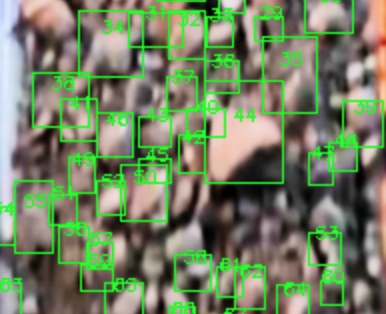
\includegraphics[width=0.6\linewidth]{images/centroid_ids}
	\caption{Отслеживание с присвоение идентификаторов с использованием корреляционного и центроидного трекеров.}
	\label{fig:centroidids}
\end{figure}

Были выявлены следующие положительные стороны:
\begin{itemize}
	\item высокая скорость обработки кадра;
	\item регистрация новых объектов;
	\item удаление исчезнувших из кадра объектов.
\end{itemize}

Были выявлены следующие проблемы:
\begin{itemize}
	\item необходимость запускать детектирование новых объектов;
	\item достаточно низкая точность.
\end{itemize}

\chapterconclusion
На основе отслеживания объектов можно определить, сколько кадров требуется на то, чтобы камень прошёл по всей ленте конвейера, иными словами, раз в какое количество кадров необходимо запускать процесс детектирования. Несмотря на достаточную низкую точность, для этого процесса лучше подходит сочетание корреляционного и центроидного трекеров, так как они позволяют отслеживать конкретные объекты. В главе \ref{practic} будет рассмотрено применение трекеров для данной задачи. 

%% Макрос для заключения. Совместим со старым стилевиком.
\chapter{Практическое исследование} \label{practic}
\section{Оценка размеров камня}
Для построения распределения необходимо определить, каким образом вычислять размер камня. Существует несколько подходов к этой оценке. Рассмотрим самые популярные из них (рис. \ref{fig:stones}). 
\begin{figure}
	\centering
	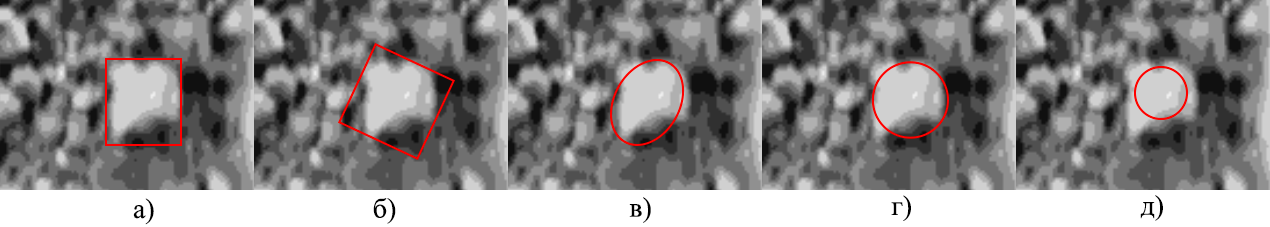
\includegraphics[width=1\linewidth]{images/stones}
	\caption{Варианты определения размера камня. а) диаметр Ферета б) оптимальный прямоугольник в) эллипс эквивалентной площади г) круг эквавалентной площади д) максимально вписываемый круг}
	\label{fig:stones}
\end{figure}

\textit{Диаметр Ферета} - минимальный прямоугольник со сторонами, параллельными осям $x$ и $y$, окружающий камень.

\textit{Оптимальный прямоугольник} - определяется как прямоугольник с наименьшей площадью, которая при любом повороте соответствует области интереса. Оптимальный прямоугольник рассчитывается путем простого определения прямоугольника площади прямоугольника, которая подходит для области, полученной поворотом на один градус.

\textit{Эллипс эквивалентной площади} - это эллипс, имеющий ту же площадь и ориентированный так же, как камень, где центр эллипса равен центру камня. Аналогично, эквивалентная площадь любой частицы - это количество пикселей в двоичном отображения. Чтобы описать размер и форму интересующей частицы, из эквивалентного эллипса извлекаются главные и второстепенные оси.

\textit{Круг эквивалнтной площади} - это круг с той же площадью, что и у частицы. Эквивалентная область любой камня определяется количеством пикселей в двоичном отображении. Диаметр эквивалентной площади круга описывает размер камня.

\textit{Максимально вписываемый круг} -  это диаметр самого большого круга, который умещается внутри камня. Он рассчитывается с использованием простого метода подбора с использованием морфологического преобразования открытия.  Реализация начинается с круга радиусом 1, и пока диск помещается внутри частицы, вычисляется круг диаметров больше текущего, пока не вычислиться максимальный диаметр. 

В данной работе оптимально использовать диаметр Ферета как наиболее просто вычисляемый, но, тем не менее, имеющий высокую точность.

\section{Оценка точности детектирования}
Наилучшие результаты показали методы водораздела и использование нейросети unet, обученной на данных водораздела. Оценим точность выполненного детектирования. 

В качестве исходных данных возмём одно и то же изображение и примененим к нему алгоритмы детектирования. 

\begin{figure}[h!]
	\begin{minipage}[h]{0.3\linewidth}
		\centering
		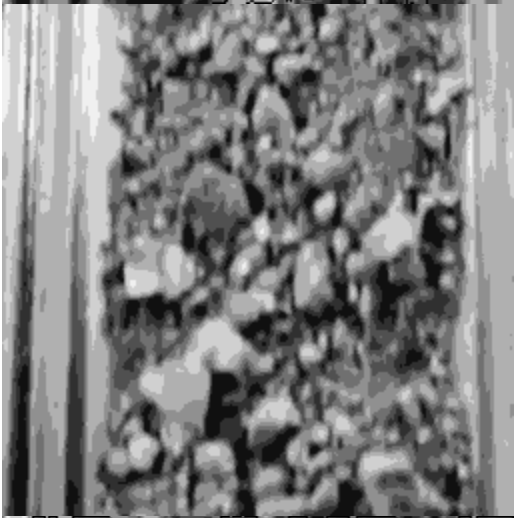
\includegraphics[width=\linewidth]{images/clear} \\ a)
	\end{minipage}
	\hfill
	\begin{minipage}[h]{0.3\linewidth}
		\centering
		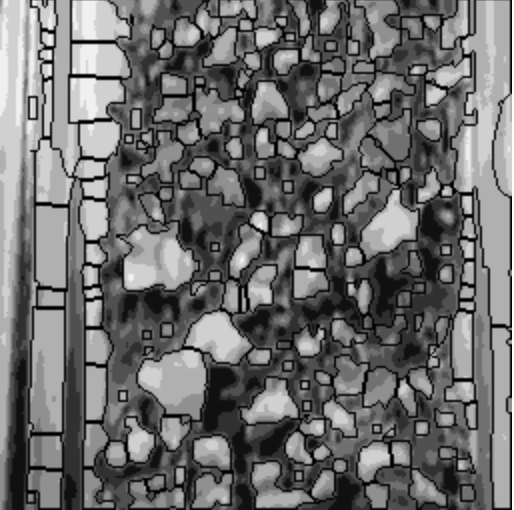
\includegraphics[width=\linewidth]{images/watersher} \\ б)
	\end{minipage}
	\hfill
	\begin{minipage}[h]{0.3\linewidth}
		\centering
		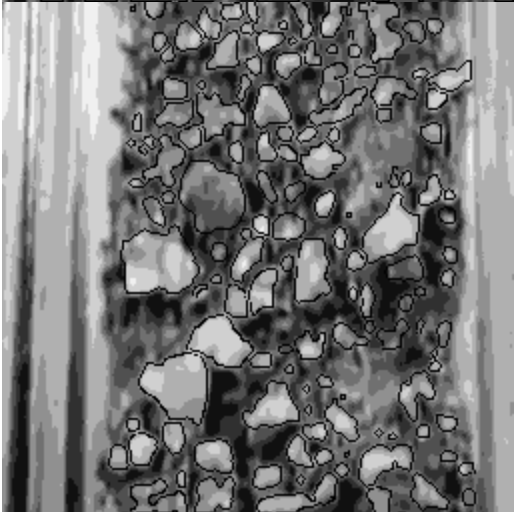
\includegraphics[width=\linewidth]{images/uner} \\в)
	\end{minipage}
	\caption{Полученные результаты. а) исходное изображение б) водораздел в) Unet}
	\label{fig:total}
\end{figure}

Сравнительный анализ работы алгоритмов представлен в таблице \ref{tab3}. Использование нейронной сети Unet позволяет достичь более точного выделения камней на ленте конвейера. Нейронная сеть позволяет сократить ошибку разграничения частиц, так как обучена таким образом, что не выделяет области песка как крупные камни(рис. \ref{fig:rasp}). Так же она не допускает выделения объектов конвейера как камни и снижает излишнюю сегментацию.
\begin{table}[!h]
	\caption{Сравнение результатов работы алгоритма}\label{tab3}
	\centering
	\begin{tabularx}{\textwidth}{|*{4}{>{\centering\arraybackslash}X|}}\hline
		- & Wateshed & Unet  & Всего\\\hline
		Ошибка разграничения частиц & 20 & 5 & 20 \\\hline
		Излишняя сегментация & 21 & 2 & 21 \\\hline
		Лишние объекты & 30 & 0 & 30 \\\hline
		Скорость (c) & 0.04 & 0.14 & - \\\hline
	\end{tabularx}
\end{table}

\begin{figure}[h!]
	\begin{minipage}[h]{0.3\linewidth}
		\centering
		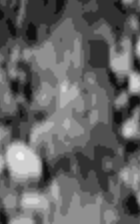
\includegraphics[width=0.5\linewidth]{images/source} \\ a)
	\end{minipage}
	\hfill
	\begin{minipage}[h]{0.3\linewidth}
		\centering
		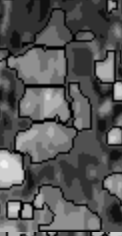
\includegraphics[width=0.5\linewidth]{images/water} \\ б)
	\end{minipage}
	\hfill
	\begin{minipage}[h]{0.3\linewidth}
		\centering
		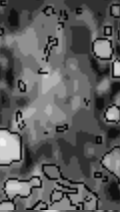
\includegraphics[width=0.5\linewidth]{images/unets} \\в)
	\end{minipage}
	\caption{Ошибка разграничения частиц. а) исходное изображение б) водораздел в) Unet}
	\label{fig:razgrl}
\end{figure}


\section{Оценка необходимой частоты построения распределения}
Целью практического эксперимента является определение расчёта количества $N$ кадров, в течение которых объект, появившийся в кадре $0$, исчезнет в кадре $N$. Будем считать скорость конвейера постоянной. Данное количество $N$  позволит определить периодичность кадров, через которые нам необходимо вычислять распределение камней по крупности, получая независимые данные. Иными словами, по результатам получится необходимое количество кадров, раз в которое нам необходимо запускать процесс детектирования, чтобы высчитывать распределение.

Единственным сочетанием трекеров, позволяющим отслеживать конкретные камни и убирать ненужные треки, является сочетанием корреляционного и центроидного трекеров. Понизим количество определяемых камней, оставив для отслеживания только крупные камни, благодаря этому мы сможем повысить точность отслеживания и сократить время обработки одного кадра.

Для отслеживания определим набор нескокльких камень с максимальным номером, присутствующим на первом из кадров. Дальнейшая задача - определить номер кадра, когда большинство из этих камней пропадут из области видимости. 

Для первого кадра  (рис. \ref{fig:frames}a) были выбраны камни 30, 31, 33, 32, 35. Автоматическое слежение показало исчезновение камня 30 в кадре \#15, камней 32, 35 в кадре \#21, так как они были неотслеживаемыми (ошибка отслеживания корреляционного трекера). Камни 31 и 33 отслеживались до \#51 кадра (рис. \ref{fig:frames}б), по истечении этого кадра они исчезли из поля зрения. Можно считать, что период прохода одного камня от начала до конца конвейера - 50 кадров. Соответственно, это будет являться частотой расчёта распределения. 
\begin{figure}[h]
	\begin{minipage}[h]{0.49\linewidth}
		\centering
		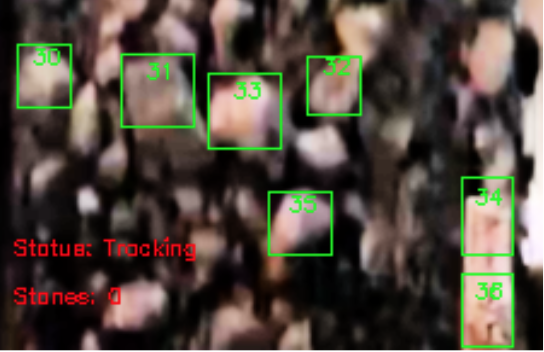
\includegraphics[width=0.8\linewidth]{images/finaltrack1} \\ a)
	\end{minipage}
	\hfill
	\begin{minipage}[h]{0.49\linewidth}
		\centering
		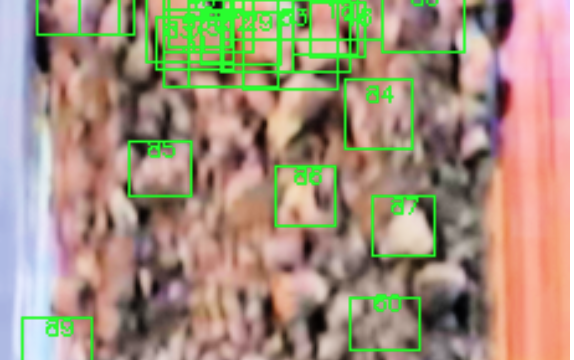
\includegraphics[width=0.8\linewidth]{images/finaltrack2} \\ б)
	\end{minipage}
	\caption{Процесс отслеживания}
	\label{fig:frames}
\end{figure}

\section{Построение распределение}

И так, по результатам детектирования камней на ленте конвейера мы можем построить диаметр Ферета (рис. \ref{fig:feret}) для каждого из камней. 
\begin{figure}[h!]
	\centering
	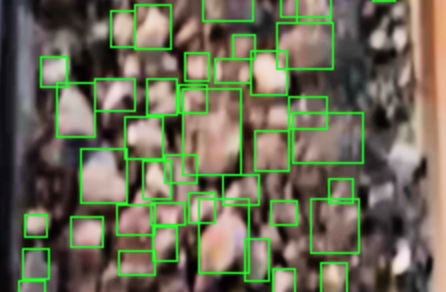
\includegraphics[width=0.4\linewidth]{images/feret}
	\caption{Построенные диаметры Ферета}
	\label{fig:feret}
\end{figure}
На основе этих данных мы можем построить гистограмма (рис. \ref{fig:rasp}), которое будет показывать распредение камней по размеру на данном участке конвейера. В качестве размера берётся  площадь полученного прямоугольника.
На построенном примере распределения мы можем видеть преобладание камней небольшой площади. На основе накопленных данных распредения определяются пороговые значения размеров камней, по котором можно определять крупность для управления мельницей.

\begin{figure}[h]
	\begin{minipage}[h]{0.49\linewidth}
		\centering
		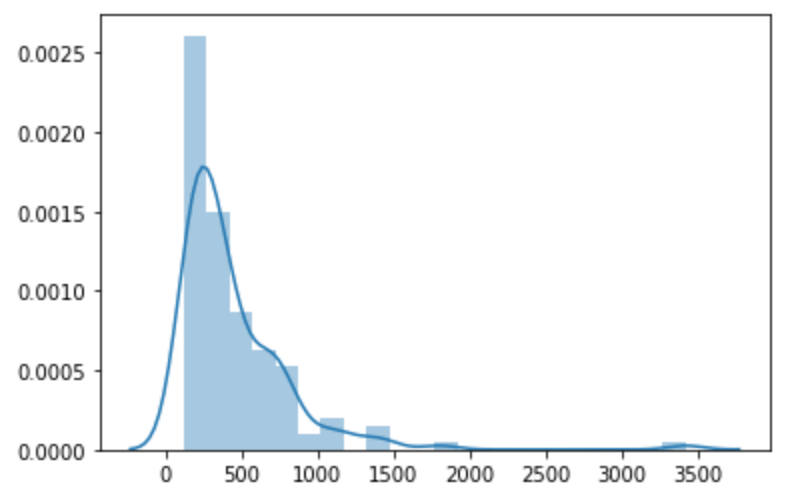
\includegraphics[width=0.8\linewidth]{images/raspr} \\ a)
	\end{minipage}
	\hfill
	\begin{minipage}[h]{0.49\linewidth}
		\centering
		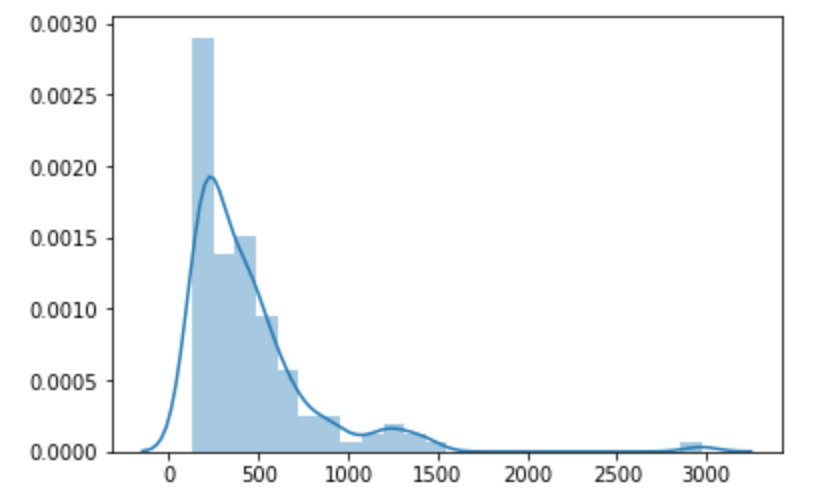
\includegraphics[width=0.8\linewidth]{images/raspr2} \\ б)
	\end{minipage}
	\caption{Построенное распределение.}
	\label{fig:rasp}
\end{figure}


\chapterconclusion
В данной главе были проведены практические эксперименты, демонстрирующие численные результаты работы методов детектирования - алгоритмов водораздела и применения обученной нейронной сети. Показана эффективность применения нейронной сети Unet для детектирования камней на конвейере. Вычислена периодичность построения распределения и построено распределение камней по конвейеру.


\startconclusionpage
В ходе данной работы были исследованы методы автоматизации управления мельницей для обработки руды с помощью компьютерного зрения, а именно решение задачи автоматического гранулометрического анализа. Управление мельницей в настоящий момент происходит вручную, что может привести к неэффективному режиму работы.

Самой сложной задачей в автоматизации гранулометрии является детектирование камней.

Были исследовано применение классических методов компьютерного зрения - различных методов определения границ, метод водораздела, основанный на приниципе выращивания регионов, однако лучший из классических методов - метод водораздела показал точность 54\%, что не является достаточным.

Так же было исследовано применения методов оптического потока для детектирования камней - как разреженого, так и плотного (методы Лукаса-Канаде, Фарнэбека, SimpleFlow), но их использование по результатам экспериментов были признано неэффективным.

Наилучший результат детектированиия показало использование нейронной сети Unet, предназначенной для семантической сегментации изображений. Нейронная сеть была обучена на выборке, созданной с помощью метода водораздела, скорректированного вручную.

Так же стояла задача определить необходимую периодичность вычисления. Для этого были исследованы различных методы отслеживания (трекер на основе алгоритма обучения на нескольких экземплярах, корреляционный трекер, центроидный трекер). Лучший результат показало сочетание корреляционного и центроидного трекеров, с помощью которых получилось определить необходимую периодичность кадров. 
Задачи исследования выполнены в полном объеме. Поставленная в начале исследования цель достигнута.

%% Обратите внимание на heading. Без него тоже работает, но название будет другим.
\printmainbibliography

%% После этой команды chapter будет генерировать приложения, нумерованные русскими буквами.
%% \startappendices из старого стилевика будет делать то же самое
\appendix

\chapter{Реализация детектирования метода водораздела}
 \begin{lstlisting}[caption={Метод водораздела},label={lstX}]
 
 import numpy as np
 import cv2
 from google.colab.patches import cv2_imshow
 from skimage.feature import peak_local_max
 from skimage.morphology import watershed
 from scipy import ndimage
 import imutils
 import random as rand
 import numpy as np
 from datetime import datetime
 import time
 
 cap = cv2.VideoCapture('IMG_0573.MOV')
 # while(cap.isOpened()):
 
 """#Preprocessing"""
 
 def crop(frame):
 return frame[128:384, 0:256]
 
 def preprocessing(frame):
 frame = frame[0:700, 100:370]
 frame = cv2.GaussianBlur(frame,(3,3),0)
 
 hsv = cv2.cvtColor(frame, cv2.COLOR_BGR2HSV)
 h, s, v = cv2.split(hsv)
 
 v = cv2.equalizeHist(v)
 
 hsv = cv2.merge([h, s, v])
 bgr = cv2.cvtColor(hsv, cv2.COLOR_HSV2BGR)
 gray = cv2.cvtColor(bgr, cv2.COLOR_BGR2GRAY)
 div = 32
 gray = gray // div * div + div // 2
 
 return bgr, gray
 
 def doOpening(frame):
 kernel = np.ones((5,5),np.uint8)
 frame = cv2.morphologyEx(frame, cv2.MORPH_OPEN, kernel)
 frame = cv2.equalizeHist(frame)
 return frame
 
 def getSobel(v):
 scale = 1
 delta = 0
 ddepth = cv2.CV_16S
 grad_x = cv2.Sobel(v, ddepth, 1, 0, ksize=3, scale=scale, delta=delta, borderType=cv2.BORDER_DEFAULT)
 # Gradient-Y
 # grad_y = cv.Scharr(gray,ddepth,0,1)
 grad_y = cv2.Sobel(v, ddepth, 0, 1, ksize=3, scale=scale, delta=delta, borderType=cv2.BORDER_DEFAULT)
 
 abs_grad_x = cv2.convertScaleAbs(grad_x)
 abs_grad_y = cv2.convertScaleAbs(grad_y)
 maskSobel = cv2.addWeighted(abs_grad_x, 0.5, abs_grad_y, 0.5, 0)
 return maskSobel
 
 def findMarkers(v):
 kernel = np.ones((5,5),np.uint8)
 v = cv2.morphologyEx(v, cv2.MORPH_OPEN, kernel)
 v = cv2.equalizeHist(v)
 thresh = cv2.adaptiveThreshold(v,255,cv2.ADAPTIVE_THRESH_MEAN_C,\
 cv2.THRESH_BINARY,39,2)
 return thresh
 
 def doWatershed(thresh, mask):
 distance_map = ndimage.distance_transform_edt(thresh)
 local_max = peak_local_max(distance_map, indices=False, min_distance=5, labels=thresh)
 # Perform connected component analysis then apply Watershed
 markers = ndimage.label(local_max, structure=np.ones((3, 3)))[0]
 labels = watershed(-distance_map, markers, mask=thresh)
 return labels
 
 def getRectangle(cont):
 minX = np.min(cont[:,0,0])
 minY = np.min(cont[:,0,1])
 maxX = np.max(cont[:,0,0])
 maxY = np.max(cont[:,0,1])
 if (5 < maxX-minX < 100) and (5 < maxY-minY < 100):
 currentStone = (minX, minY, maxX-minX, maxY-minY)
 #currentStone = np.array([[[minX, minY]], [[minX, maxY]], [[maxX, maxY]], [[maxX, minY]]], dtype=np.int32)
 return currentStone
 else:
 return None
 
 def findContours_rect(gray):
 
 markers = findMarkers(gray)
 
 # Iterate through unique labels
 labels = doWatershed(markers)
 
 n = 0
 Areas = []
 rects = []
 for label in np.unique(labels):
 if label == 0:
 continue
 # Create a mask
 mask = np.zeros(markers.shape, dtype="uint8")
 mask[labels == label] = 255
 
 # Find contours and determine contour area
 cnts = cv2.findContours(mask.copy(), cv2.RETR_EXTERNAL, cv2.CHAIN_APPROX_SIMPLE)
 cnts = cnts[0] if len(cnts) == 2 else cnts[1]
 c = max(cnts, key=cv2.contourArea)
 rect = getRectangle(c)
 if rect:
 rects.append(rect)
 return rects
 
 def findContoursOnMask(gray):
 
 markers = findMarkers(gray)
 
 # Iterate through unique labels
 labels = doWatershed(markers)
 
 n = 0
 Areas = []
 rects = []
 for label in np.unique(labels):
 if label == 0:
 continue
 # Create a mask
 mask = np.zeros(markers.shape, dtype="uint8")
 mask[labels == label] = 255
 
 # Find contours and determine contour area
 cnts = cv2.findContours(mask.copy(), cv2.RETR_EXTERNAL, cv2.CHAIN_APPROX_SIMPLE)
 cnts = cnts[0] if len(cnts) == 2 else cnts[1]
 c = max(cnts, key=cv2.contourArea)
 rect = getRectangle(c)
 if rect:
 rects.append(rect)
 return rects
 
 def findContours(gray, mode=3, returnContours=False):
 
 markers = findMarkers(gray)
 
 maskSobel = getSobel(gray)
 # Iterate through unique labels
 labels = doWatershed(markers, maskSobel)
 
 black=np.zeros(gray.shape, np.uint8)
 
 n = 0
 Areas = []
 contours = []
 for label in np.unique(labels):
 if label == 0:
 continue
 # Create a mask
 mask = np.zeros(markers.shape, dtype="uint8")
 mask[labels == label] = 255
 # Find contours and determine contour area
 cnts = cv2.findContours(mask.copy(), cv2.RETR_EXTERNAL, cv2.CHAIN_APPROX_SIMPLE)
 cnts = cnts[0] if len(cnts) == 2 else cnts[1]
 c = max(cnts, key=cv2.contourArea)
 contours.append(c)
 area = cv2.contourArea(c)
 if area>10:
 Areas.append(area)
 n+=1
 if mode==0:
 cv2.drawContours(black,[c],-1,(255, 255, 255), -1)
 if mode==1:
 cv2.drawContours(black,[c],-1,(0, 0, 0), 1)
 if mode==2:
 cv2.drawContours(black,[c],-1,(255, 255, 255), -1)
 cv2.drawContours(black,[c],-1,(0, 0, 0), 1)
 if mode==3:
 cv2.drawContours(gray,[c],-1,(0, 0, 0), 1)
 if returnContours:
 return contours
 else:
 return gray, black
 
 def drawContours(contours, real):
 cv2.drawContours(real, contours, -1, (0,200,0), -1)
 
 """#Detecting"""
 
 !git clone https://github.com/zhixuhao/unet
 
 !rm ./unet/data/membrane/train/image/*
 
 !rm /content/unet/data/membrane/test/*
 
 !rm ./unet/data/membrane/train/label/*
 
 !rm ./unet/data/membrane/train/aug/*
 
 # while(cap.isOpened()):
 cap = cv2.VideoCapture('IMG_0573.MOV')
 for i in range(10):
 for j in range(5):
 ret, frame = cap.read()
 start_time = datetime.now()
 ret, frame = cap.read()
 
 bgr, gray = preprocessing(frame)
 gray = crop(gray)
 cv2_imshow(gray)
 gray, result = findContours(gray, 2)
 print(datetime.now()-start_time)
 cv2_imshow(result)
 
 cv2.imwrite('./unet/data/membrane/train/image/'+str(i)+'.png', gray)
 # cv2.imwrite('./unet/data/membrane/train/label/'+str(i)+'.png', result)
  \end{lstlisting}
  
  
  \chapter{Реализация нейронной сети Unet}
  \begin{lstlisting}[caption={Реализация сети Unet},label={lstX}]
  
  import numpy as np 
  import os
  import skimage.io as io
  import skimage.transform as trans
  import numpy as np
  from keras.models import *
  from keras.layers import *
  from keras.optimizers import *
  from keras.callbacks import ModelCheckpoint, LearningRateScheduler
  from keras import backend as keras
  
  
  def unet(pretrained_weights = None,input_size = (256,256,1)):
  inputs = Input(input_size)
  conv1 = Conv2D(64, 3, activation = 'relu', padding = 'same', kernel_initializer = 'he_normal')(inputs)
  conv1 = Conv2D(64, 3, activation = 'relu', padding = 'same', kernel_initializer = 'he_normal')(conv1)
  pool1 = MaxPooling2D(pool_size=(2, 2))(conv1)
  conv2 = Conv2D(128, 3, activation = 'relu', padding = 'same', kernel_initializer = 'he_normal')(pool1)
  conv2 = Conv2D(128, 3, activation = 'relu', padding = 'same', kernel_initializer = 'he_normal')(conv2)
  pool2 = MaxPooling2D(pool_size=(2, 2))(conv2)
  conv3 = Conv2D(256, 3, activation = 'relu', padding = 'same', kernel_initializer = 'he_normal')(pool2)
  conv3 = Conv2D(256, 3, activation = 'relu', padding = 'same', kernel_initializer = 'he_normal')(conv3)
  pool3 = MaxPooling2D(pool_size=(2, 2))(conv3)
  conv4 = Conv2D(512, 3, activation = 'relu', padding = 'same', kernel_initializer = 'he_normal')(pool3)
  conv4 = Conv2D(512, 3, activation = 'relu', padding = 'same', kernel_initializer = 'he_normal')(conv4)
  drop4 = Dropout(0.5)(conv4)
  pool4 = MaxPooling2D(pool_size=(2, 2))(drop4)
  
  conv5 = Conv2D(1024, 3, activation = 'relu', padding = 'same', kernel_initializer = 'he_normal')(pool4)
  conv5 = Conv2D(1024, 3, activation = 'relu', padding = 'same', kernel_initializer = 'he_normal')(conv5)
  drop5 = Dropout(0.5)(conv5)
  
  up6 = Conv2D(512, 2, activation = 'relu', padding = 'same', kernel_initializer = 'he_normal')(UpSampling2D(size = (2,2))(drop5))
  merge6 = concatenate([drop4,up6], axis = 3)
  conv6 = Conv2D(512, 3, activation = 'relu', padding = 'same', kernel_initializer = 'he_normal')(merge6)
  conv6 = Conv2D(512, 3, activation = 'relu', padding = 'same', kernel_initializer = 'he_normal')(conv6)
  
  up7 = Conv2D(256, 2, activation = 'relu', padding = 'same', kernel_initializer = 'he_normal')(UpSampling2D(size = (2,2))(conv6))
  merge7 = concatenate([conv3,up7], axis = 3)
  conv7 = Conv2D(256, 3, activation = 'relu', padding = 'same', kernel_initializer = 'he_normal')(merge7)
  conv7 = Conv2D(256, 3, activation = 'relu', padding = 'same', kernel_initializer = 'he_normal')(conv7)
  
  up8 = Conv2D(128, 2, activation = 'relu', padding = 'same', kernel_initializer = 'he_normal')(UpSampling2D(size = (2,2))(conv7))
  merge8 = concatenate([conv2,up8], axis = 3)
  conv8 = Conv2D(128, 3, activation = 'relu', padding = 'same', kernel_initializer = 'he_normal')(merge8)
  conv8 = Conv2D(128, 3, activation = 'relu', padding = 'same', kernel_initializer = 'he_normal')(conv8)
  
  up9 = Conv2D(64, 2, activation = 'relu', padding = 'same', kernel_initializer = 'he_normal')(UpSampling2D(size = (2,2))(conv8))
  merge9 = concatenate([conv1,up9], axis = 3)
  conv9 = Conv2D(64, 3, activation = 'relu', padding = 'same', kernel_initializer = 'he_normal')(merge9)
  conv9 = Conv2D(64, 3, activation = 'relu', padding = 'same', kernel_initializer = 'he_normal')(conv9)
  conv9 = Conv2D(2, 3, activation = 'relu', padding = 'same', kernel_initializer = 'he_normal')(conv9)
  conv10 = Conv2D(1, 1, activation = 'sigmoid')(conv9)
  
  model = Model(input = inputs, output = conv10)
  
  model.compile(optimizer = Adam(lr = 1e-4), loss = 'binary_crossentropy', metrics = ['accuracy'])
  
  #model.summary()
  
  if(pretrained_weights):
  model.load_weights(pretrained_weights)
  
  return model
  
  from __future__ import print_function
  from keras.preprocessing.image import ImageDataGenerator
  import numpy as np 
  import os
  import glob
  import skimage.io as io
  import skimage.transform as trans
  
  Sky = [128,128,128]
  Building = [128,0,0]
  Pole = [192,192,128]
  Road = [128,64,128]
  Pavement = [60,40,222]
  Tree = [128,128,0]
  SignSymbol = [192,128,128]
  Fence = [64,64,128]
  Car = [64,0,128]
  Pedestrian = [64,64,0]
  Bicyclist = [0,128,192]
  Unlabelled = [0,0,0]
  
  COLOR_DICT = np.array([Sky, Building, Pole, Road, Pavement,
  Tree, SignSymbol, Fence, Car, Pedestrian, Bicyclist, Unlabelled])
  
  
  def adjustData(img,mask,flag_multi_class,num_class):
  if(flag_multi_class):
  img = img / 255
  mask = mask[:,:,:,0] if(len(mask.shape) == 4) else mask[:,:,0]
  new_mask = np.zeros(mask.shape + (num_class,))
  for i in range(num_class):
  #for one pixel in the image, find the class in mask and convert it into one-hot vector
  #index = np.where(mask == i)
  #index_mask = (index[0],index[1],index[2],np.zeros(len(index[0]),dtype = np.int64) + i) if (len(mask.shape) == 4) else (index[0],index[1],np.zeros(len(index[0]),dtype = np.int64) + i)
  #new_mask[index_mask] = 1
  new_mask[mask == i,i] = 1
  new_mask = np.reshape(new_mask,(new_mask.shape[0],new_mask.shape[1]*new_mask.shape[2],new_mask.shape[3])) if flag_multi_class else np.reshape(new_mask,(new_mask.shape[0]*new_mask.shape[1],new_mask.shape[2]))
  mask = new_mask
  elif(np.max(img) > 1):
  img = img / 255
  mask = mask /255
  mask[mask > 0.5] = 1
  mask[mask <= 0.5] = 0
  return (img,mask)
  
  
  
  def trainGenerator(batch_size,train_path,image_folder,mask_folder,aug_dict,image_color_mode = "grayscale",
  mask_color_mode = "grayscale",image_save_prefix  = "image",mask_save_prefix  = "mask",
  flag_multi_class = False,num_class = 2,save_to_dir = None,target_size = (256,256),seed = 1):
  '''
  can generate image and mask at the same time
  use the same seed for image_datagen and mask_datagen to ensure the transformation for image and mask is the same
  if you want to visualize the results of generator, set save_to_dir = "your path"
  '''
  image_datagen = ImageDataGenerator(**aug_dict)
  mask_datagen = ImageDataGenerator(**aug_dict)
  image_generator = image_datagen.flow_from_directory(
  train_path,
  classes = [image_folder],
  class_mode = None,
  color_mode = image_color_mode,
  target_size = target_size,
  batch_size = batch_size,
  save_to_dir = save_to_dir,
  save_prefix  = image_save_prefix,
  seed = seed)
  mask_generator = mask_datagen.flow_from_directory(
  train_path,
  classes = [mask_folder],
  class_mode = None,
  color_mode = mask_color_mode,
  target_size = target_size,
  batch_size = batch_size,
  save_to_dir = save_to_dir,
  save_prefix  = mask_save_prefix,
  seed = seed)
  train_generator = zip(image_generator, mask_generator)
  for (img,mask) in train_generator:
  img,mask = adjustData(img,mask,flag_multi_class,num_class)
  yield (img,mask)
  
  
  
  def testGenerator(test_path,num_image = 30,target_size = (256,256),flag_multi_class = False,as_gray = True):
  for i in range(num_image):
  img = io.imread(os.path.join(test_path,"%d.png"%i),as_gray = as_gray)
  img = img / 255
  img = trans.resize(img,target_size)
  img = np.reshape(img,img.shape+(1,)) if (not flag_multi_class) else img
  img = np.reshape(img,(1,)+img.shape)
  yield img
  
  
  def geneTrainNpy(image_path,mask_path,flag_multi_class = False,num_class = 2,image_prefix = "image",mask_prefix = "mask",image_as_gray = True,mask_as_gray = True):
  image_name_arr = glob.glob(os.path.join(image_path,"%s*.png"%image_prefix))
  image_arr = []
  mask_arr = []
  for index,item in enumerate(image_name_arr):
  img = io.imread(item,as_gray = image_as_gray)
  img = np.reshape(img,img.shape + (1,)) if image_as_gray else img
  mask = io.imread(item.replace(image_path,mask_path).replace(image_prefix,mask_prefix),as_gray = mask_as_gray)
  mask = np.reshape(mask,mask.shape + (1,)) if mask_as_gray else mask
  img,mask = adjustData(img,mask,flag_multi_class,num_class)
  image_arr.append(img)
  mask_arr.append(mask)
  image_arr = np.array(image_arr)
  mask_arr = np.array(mask_arr)
  return image_arr,mask_arr
  
  
  def labelVisualize(num_class,color_dict,img):
  img = img[:,:,0] if len(img.shape) == 3 else img
  img_out = np.zeros(img.shape + (3,))
  for i in range(num_class):
  img_out[img == i,:] = color_dict[i]
  return img_out / 255
  
  
  
  def saveResult(save_path,npyfile,flag_multi_class = False,num_class = 2):
  for i,item in enumerate(npyfile):
  img = labelVisualize(num_class,COLOR_DICT,item) if flag_multi_class else item[:,:,0]
  io.imsave(os.path.join(save_path,"%d_predict.png"%i),img)
  data_gen_args = dict(rotation_range=0.2,
  width_shift_range=0.05,
  height_shift_range=0.05,
  shear_range=0.05,
  zoom_range=0.05,
  horizontal_flip=True,
  fill_mode='nearest')
  myGene = trainGenerator(2,'/content/unet/data/membrane/train','image','label',data_gen_args,save_to_dir = None)
  model = unet()
  model_checkpoint = ModelCheckpoint('unet_membrane.hdf5', monitor='loss',verbose=1, save_best_only=True)
  model.fit_generator(myGene,steps_per_epoch=2000,epochs=5,callbacks=[model_checkpoint])
  \end{lstlisting}
  
    \chapter{Реализация отслеживания с использованием корреляционного и центроидного трекера}
  \begin{lstlisting}[caption={Корреляционный и центроидный трекер},label={lstX}]
  class TrackableObject:
	  def __init__(self, objectID, centroid):
		  # store the object ID, then initialize a list of centroids
		  # using the current centroid
		  self.objectID = objectID
		  self.centroids = [centroid]
		  
		  # initialize a boolean used to indicate if the object has
		  # already been counted or not
		  self.counted = False
	# import the necessary packages
	from scipy.spatial import distance as dist
	from collections import OrderedDict
	import numpy as np
	
	class CentroidTracker:
	def __init__(self, maxDisappeared=5, maxDistance=10):
	self.nextObjectID = 0
	self.objects = OrderedDict()
	self.disappeared = OrderedDict()
	
	self.maxDisappeared = maxDisappeared
	
	
	self.maxDistance = maxDistance
	
	def register(self, centroid):
	self.objects[self.nextObjectID] = centroid
	self.disappeared[self.nextObjectID] = 0
	self.nextObjectID += 1
	
	def deregister(self, objectID):
	del self.objects[objectID]
	del self.disappeared[objectID]
	
	def update(self, rects):
	if len(rects) == 0:
	for objectID in list(self.disappeared.keys()):
	self.disappeared[objectID] += 1
	
	if self.disappeared[objectID] > self.maxDisappeared:
	self.deregister(objectID)
	
	return self.objects
	
	inputCentroids = np.zeros((len(rects), 2), dtype="int")
	
	for (i, (startX, startY, endX, endY)) in enumerate(rects):
	cX = int((startX + endX) / 2.0)
	cY = int((startY + endY) / 2.0)
	inputCentroids[i] = (cX, cY)
	
	if len(self.objects) == 0:
	for i in range(0, len(inputCentroids)):
	self.register(inputCentroids[i])
	
	else:
	objectIDs = list(self.objects.keys())
	objectCentroids = list(self.objects.values())
	
	D = dist.cdist(np.array(objectCentroids), inputCentroids)
	
	rows = D.min(axis=1).argsort()
	
	cols = D.argmin(axis=1)[rows]
	
	usedRows = set()
	usedCols = set()
	
	
	for (row, col) in zip(rows, cols):
	if row in usedRows or col in usedCols:
	continue
	if D[row, col] > self.maxDistance:
	continue
	
	objectID = objectIDs[row]
	self.objects[objectID] = inputCentroids[col]
	self.disappeared[objectID] = 0
	
	usedRows.add(row)
	usedCols.add(col)
	
	unusedRows = set(range(0, D.shape[0])).difference(usedRows)
	unusedCols = set(range(0, D.shape[1])).difference(usedCols)
	
	if D.shape[0] >= D.shape[1]:
	for row in unusedRows:
	objectID = objectIDs[row]
	self.disappeared[objectID] += 1
	
	if self.disappeared[objectID] > self.maxDisappeared:
	self.deregister(objectID)
	
	else:
	for col in unusedCols:
	self.register(inputCentroids[col])
	
	return self.objects
	
	import dlib
	from datetime import datetime
	import time
	import seaborn as sns
	import matplotlib.pyplot as plt
	
	ct = CentroidTracker(maxDisappeared=5, maxDistance=5)
	trackers = []
	# trackers = cv2.MultiTracker_create()
	trackableObjects = {}
	cap = cv2.VideoCapture('IMG_0573.MOV')
	totalFrames = 0
	totalStones = 0
	totalBig = 0
	totalSmall = 0
	%matplotlib inline
	
	
	# while True:
	maxId = 0
	for i in range(150):
	start_time = datetime.now()
	ret, frame = cap.read()
	frame, gray = preprocessing(frame)
	
	
	if frame is None:
	break
	status = "Waiting"
	rects = []
	
	if totalFrames%15 == 0:
	sizes = []
	start_detecting_time = datetime.now()
	
	status = "Detecting"
	trackers = []
	#  trackers = cv2.MultiTracker_create()
	boxes = findContours(gray)
	for box in boxes:
	(x, y, w, h) = [int(v) for v in box]
	tracker = dlib.correlation_tracker()
	rect = dlib.rectangle(x, y, x + w, y + h)
	sizes.append(max(w,h))
	tracker.start_track(frame, rect)
	trackers.append(tracker)
	# tracker = OPENCV_OBJECT_TRACKERS["mil"]()
	# trackers.add(tracker, frame, box)
	print("Detecting: ", datetime.now() - start_detecting_time)
	if(totalFrames == 1):
	maxId = max(objects.keys())
	print(maxId)
	sns.distplot(sizes)
	plt.show()
	
	else:
	for tracker in trackers:
	status = "Tracking"
	tracker.update(gray)
	pos = tracker.get_position()
	startX = int(pos.left())
	startY = int(pos.top())
	endX = int(pos.right())
	endY = int(pos.bottom())
	rects.append((startX, startY, endX, endY))
	cv2.rectangle(frame, (startX, startY), (endX, endY), (0, 0, 0), 1)
	objects = ct.update(rects)
	
	# if(maxId not in objects.keys() and totalFrames>1):
	#   print(totalFrames)
	#   break
	
	for (objectID, centroid) in objects.items():
	to = trackableObjects.get(objectID, None)
	
	# if there is no existing trackable object, create one
	if to is None:
	to = TrackableObject(objectID, centroid)
	else:
	
	y = [c[1] for c in to.centroids]
	to.centroids.append(centroid)
	
	# check to see if the object has been counted or not
	if not to.counted:
	totalStones+=1 
	to.counted = True
	
	# store the trackable object in our dictionary
	trackableObjects[objectID] = to
	
	#draw both the ID of the object and the centroid of the
	#object on the output frame
	text = "{}".format(objectID)
	cv2.putText(frame, text, (centroid[0] - 5, centroid[1] - 5),
	cv2.FONT_HERSHEY_SIMPLEX, 0.3, (0, 255, 0), 1)
	cv2.circle(frame, (centroid[0], centroid[1]), 4, (0, 255, 0), -1)
	
	# construct a tuple of information we will be displaying on the
	# frame
	info = [
	("Stones", totalStones),
	("Status", status),
	]
	
	# loop over the info tuples and draw them on our frame
	for (i, (k, v)) in enumerate(info):
	text = "{}: {}".format(k, v)
	cv2.putText(frame, text, (10, 700 - ((i * 20) + 20)),
	cv2.FONT_HERSHEY_SIMPLEX, 0.3, (0, 0, 255), 1)
	
	# show the output frame
	print("Total: ", datetime.now() - start_time)
	print(totalFrames)
	cv2_imshow(frame)
	# increment the total number of frames processed thus far and
	# then update the FPS counter
	totalFrames += 1
	
	  \end{lstlisting}
\end{document}
